

\section{Results}
\label{Results}
This section describes results for both barrier and FAS controller. Starting with the results of the validation approach, followed by the vehicle behavior (i.e. speed, target gap, acceleration and energy consumption), followed by the barrier controller performance, and lastly the KPI comparison.

\subsection{Simulation Output Validation}
Simulations showed that the headway gaps converged within the 2.5 m threshold across all simulations, which figure~\ref{fig:gapmean} supports by showing the target headway gap and the mean across all simulations per \(N\). The figure highlights that the mean headway gap sits tightly around the target gap for each \(N\).\\\\
Figure~\ref{fig:theoretical max} shows that throughput remained within the theoretical maximum across all simulations. Similarly, recorded lap times showed that the lap times remained above the theoretical minimum lap when the average speed was similar to the target speed. For some vehicles the lap time was found to be lower than the minimal lap time, due to a higher average speed. 
\\\\
The energy model is validated against the Tesla Model 3 RWD WLTP consumption of 0.136 kWh/km \parencite{rosenberger2024quantifying}, as this is the only vehicle for which a citable source is available. Table~\ref{tab:vehicle_energy_filtered} shows that the mean Tesla Model 3 RWD energy consumption range from 0.072 to 0.156 kWh/km. The 0.072 kWh/km corresponds to the barrier controller, which is 47\% below the WLTP figure, whereas using the FAS controller the energy usage is 14.7\% above the WLTP figure. These opposing directions align with the hypothesis that frequent stop-and-go behavior leads to higher energy consumption, whereas cruising at constant speed with small fluctuations in acceleration results in lower energy consumption. In addition, table~\ref{tab:vehicle_energy_filtered} shows that the Audi e-tron consumes more energy per km, which aligns with the higher \(F_\text{total}\), due to the differences in vehicle specific parameters, table~\ref{vehicle specs}.  All in all, the energy model produces realistic values despite the models simplifying assumptions.
\\\\
The counted safety violations were directly compared to videos of the simulations. The videos showed only safety violations at near simultaneous arrival, which is is line with the setup of the performance indicator.  

\begin{figure}[H]
    \centering
        % Set height instead of width to make them level
        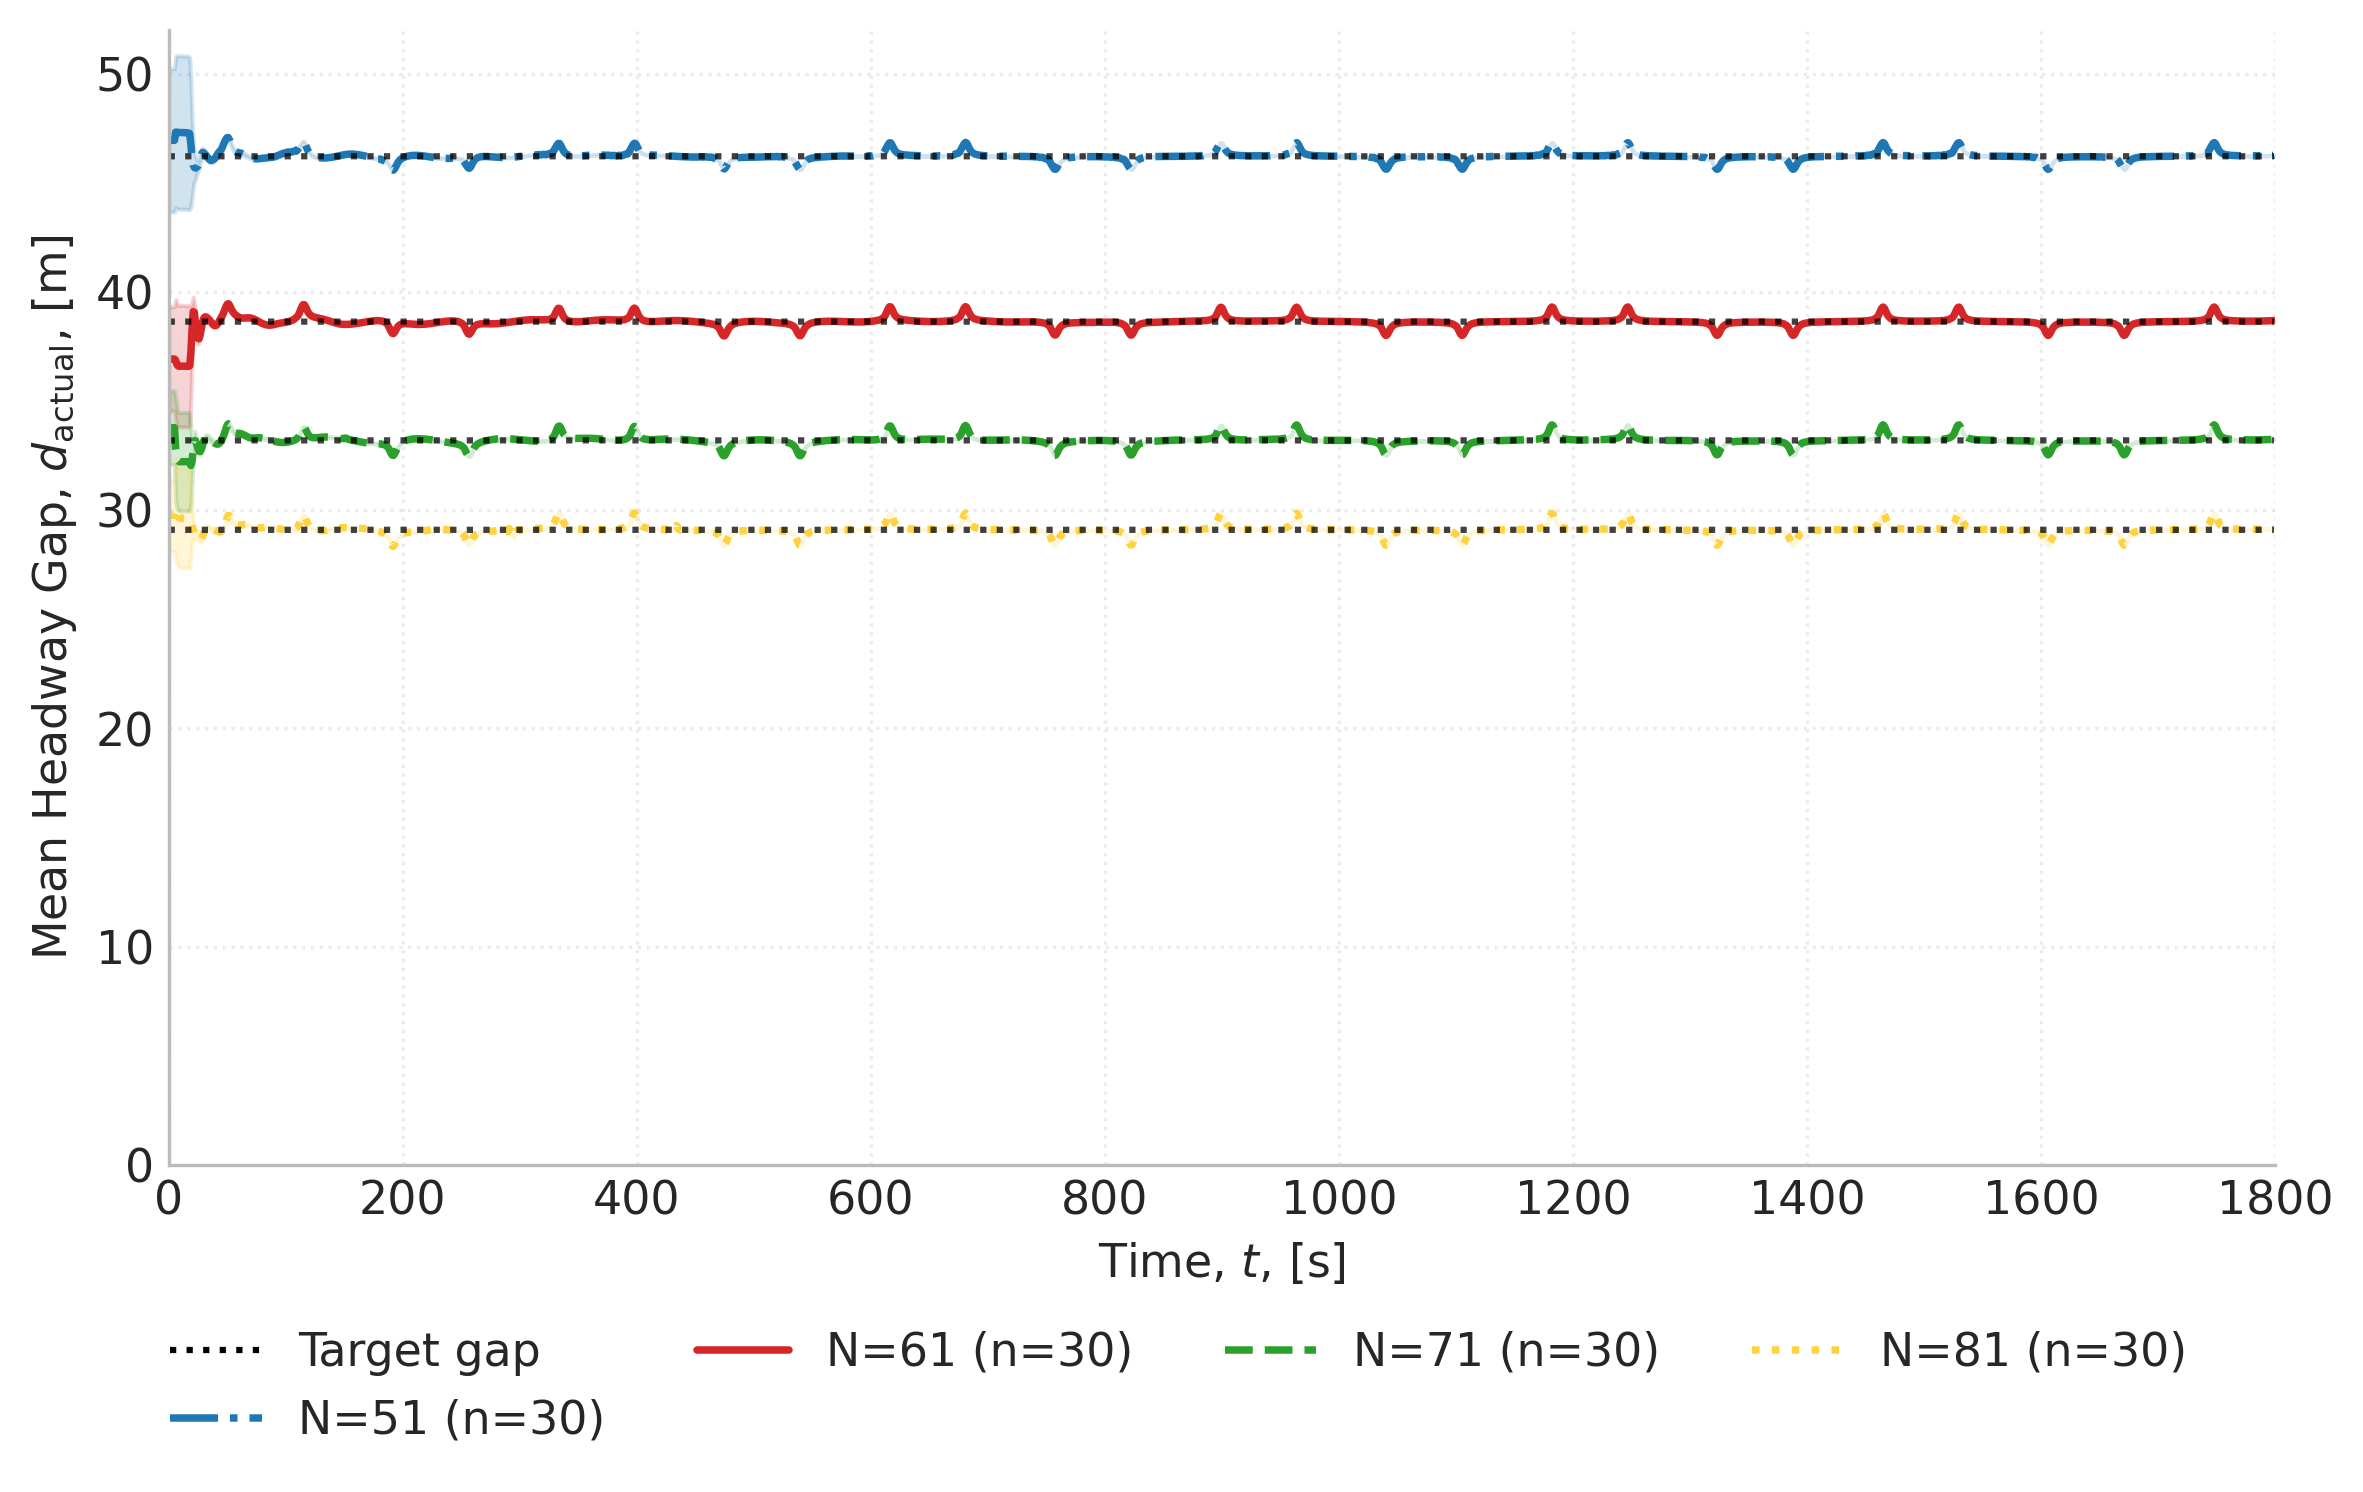
\includegraphics[ width=\linewidth, keepaspectratio]{MeanGap.png}
        \caption{Mean headway gap ± 95\% CI and target gap per vehicle density \(N = \{51,61,71,81\}\) over simulation time}
        \label{fig:gapmean}
        \end{figure}
    
    \begin{figure} [H]
        \centering
        % Set matching height here
        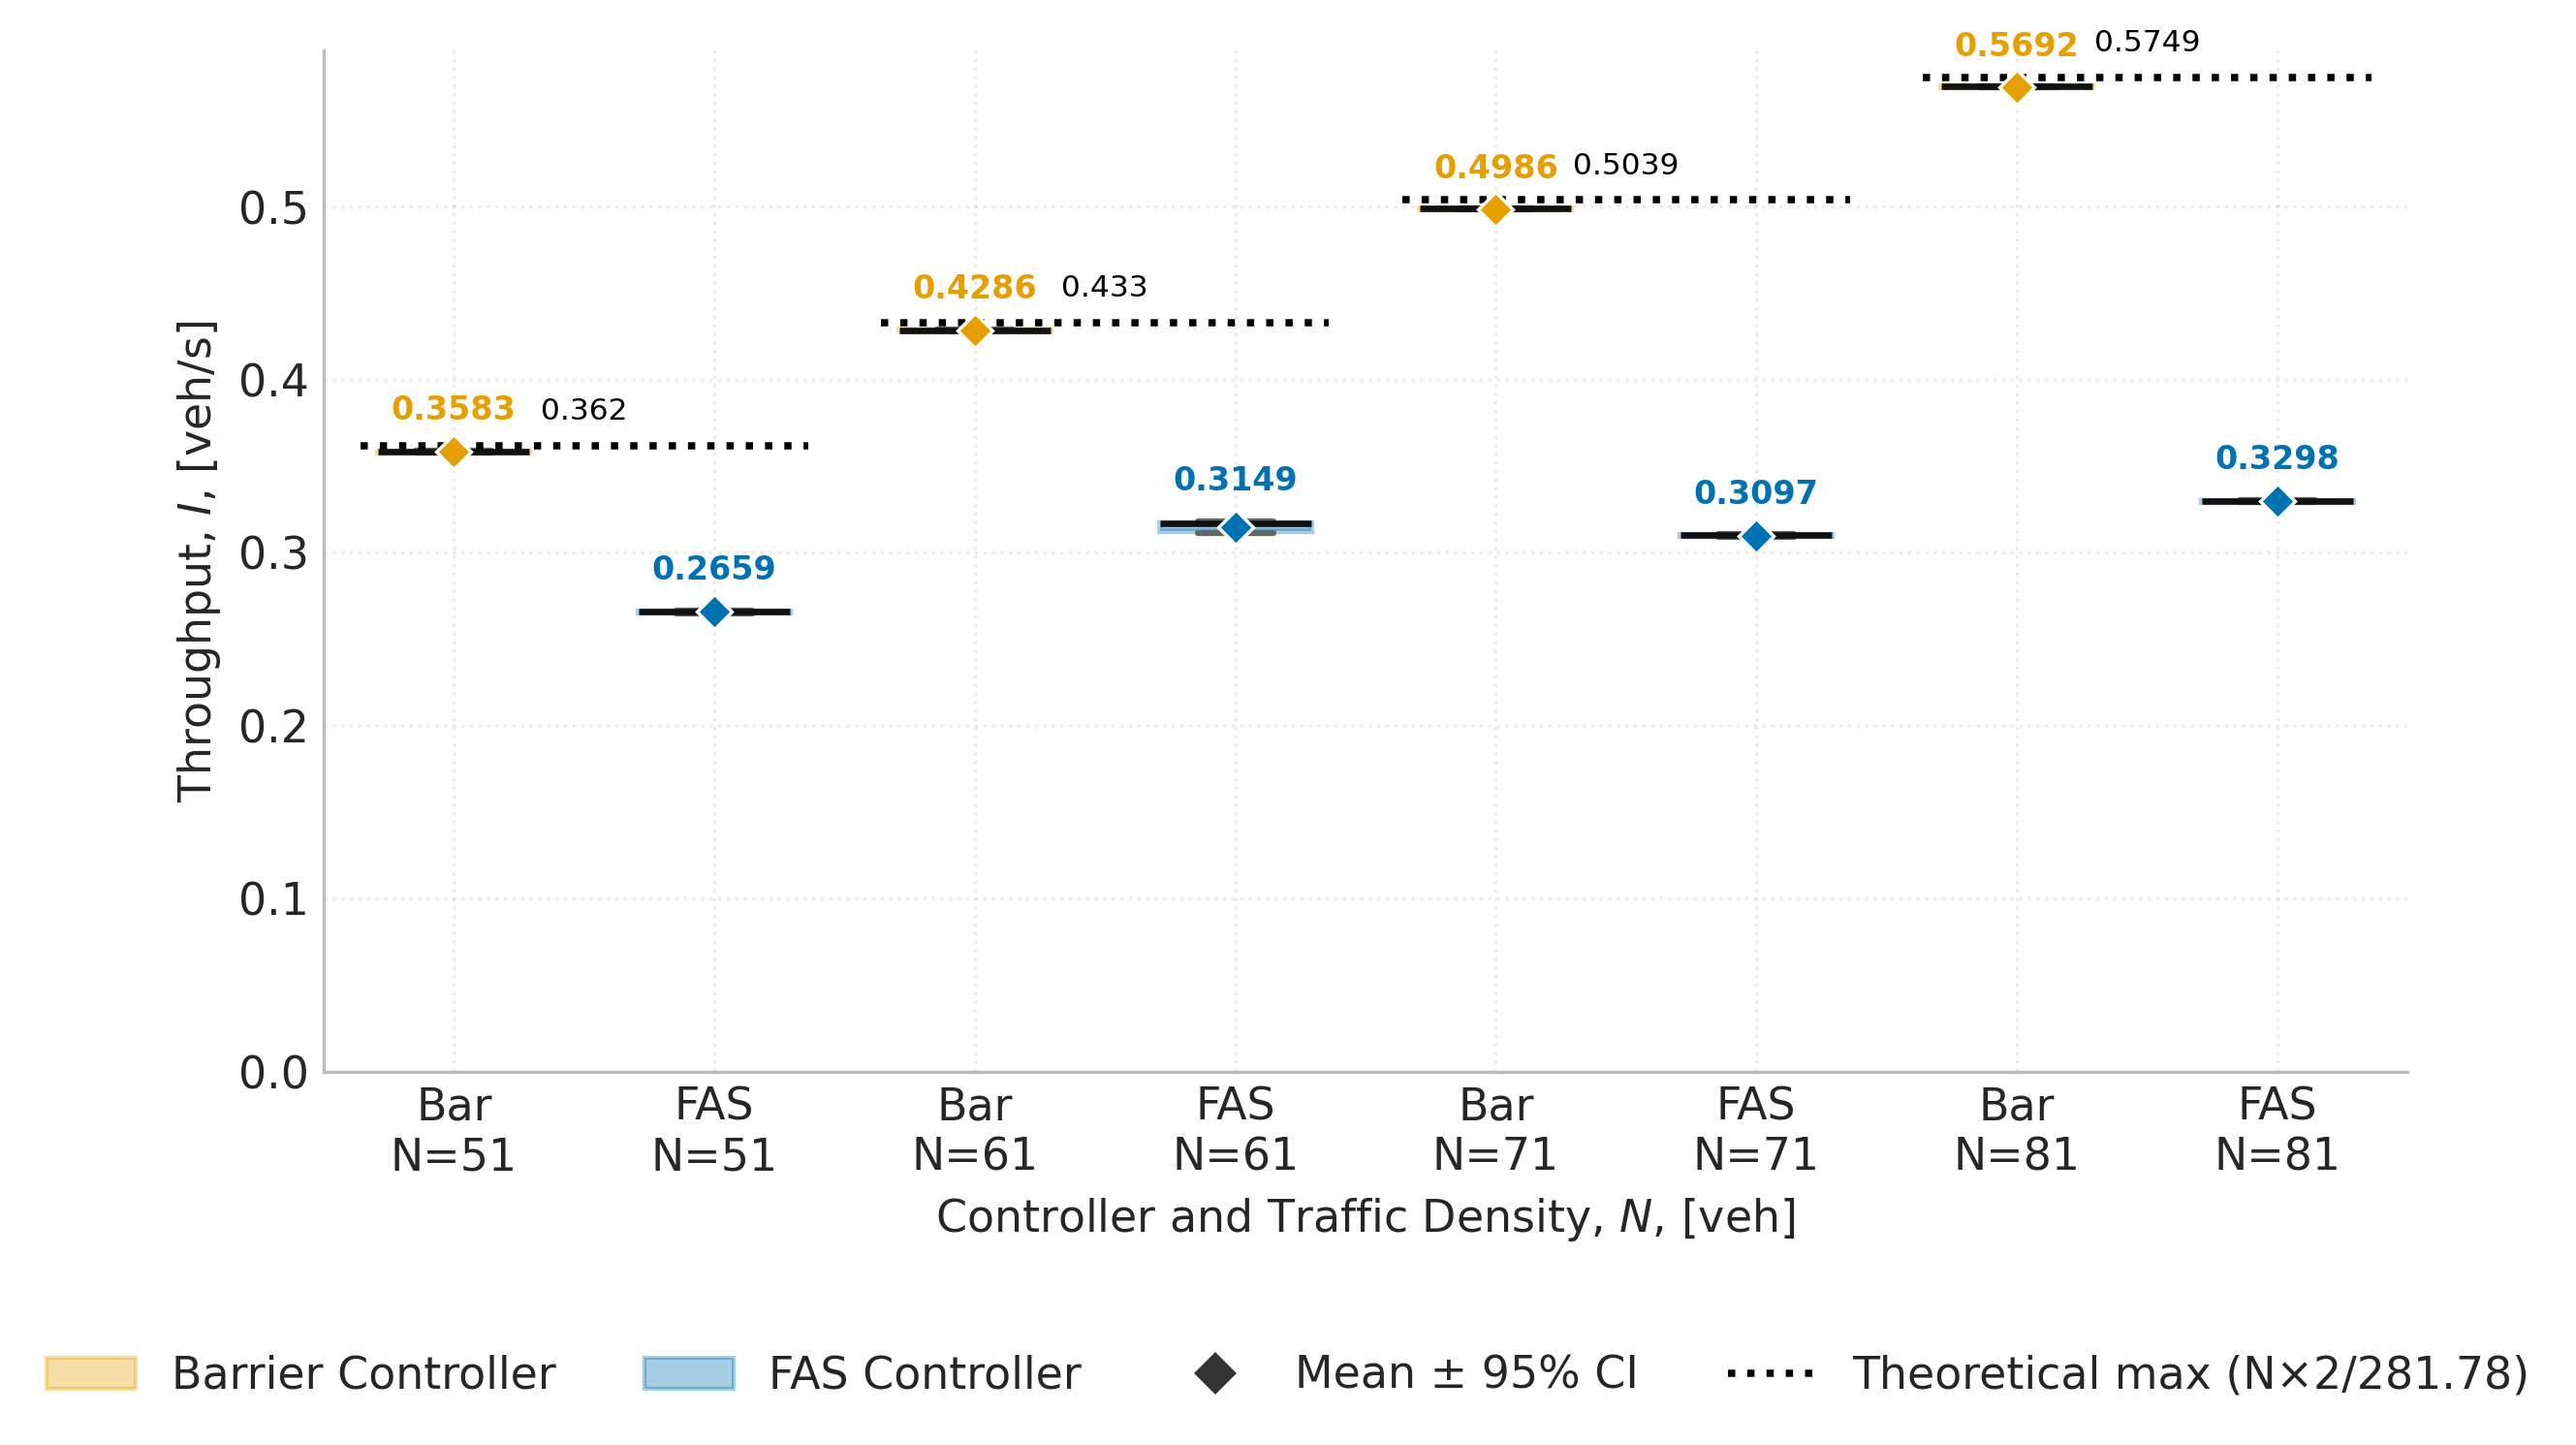
\includegraphics[ width=\linewidth, keepaspectratio]{throughput-per-demand.png}
        \caption{Boxplot with additional mean and 95\% CI per controller for each \(N\), and theoretical maximum for all \(N\)}
        \label{fig:theoretical max}
    \end{figure}

\begin{table}[H]
\centering
\caption{Vehicle Specific Energy Consumption in kWh/km, displaying mean $\pm$ 95\% CI, for all traffic densities across all controllers}
\label{tab:vehicle_energy_filtered}
\begin{tabular}{lllr}
\hline
\textbf{Controller} & \textbf{Traffic Density} & \textbf{Vehicle Type} & \textbf{Energy (kWh/km) $\pm$ 95\%CI} \\ \hline
FAS Controller     & 51 & Audi e-tron 55    & $0.139559 \pm 0.000609$ \\
FAS Controller     & 61 & Audi e-tron 55    & $0.144853 \pm 0.000474$ \\
FAS Controller     & 71 & Audi e-tron 55    & $0.181942 \pm 0.000235$ \\
FAS Controller     & 81 & Audi e-tron 55    & $0.195923 \pm 0.000393$ \\
FAS Controller     & 51 & Tesla Model 3 RWD & $0.112200 \pm 0.000489$ \\
FAS Controller     & 61 & Tesla Model 3 RWD & $0.115922 \pm 0.000438$ \\
FAS Controller     & 71 & Tesla Model 3 RWD & $0.141730 \pm 0.000158$ \\
FAS Controller     & 81 & Tesla Model 3 RWD & $0.155531 \pm 0.000238$ \\ \hline
Barrier Controller & 51 & Audi e-tron 55    & $0.089171 \pm 0.000266$ \\
Barrier Controller & 61 & Audi e-tron 55    & $0.089223 \pm 0.000309$ \\
Barrier Controller & 71 & Audi e-tron 55    & $0.089285 \pm 0.000326$ \\
Barrier Controller & 81 & Audi e-tron 55    & $0.090644 \pm 0.000288$ \\
Barrier Controller & 51 & Tesla Model 3 RWD & $0.071781 \pm 0.000196$ \\
Barrier Controller & 61 & Tesla Model 3 RWD & $0.072030 \pm 0.000387$ \\
Barrier Controller & 71 & Tesla Model 3 RWD & $0.071914 \pm 0.000294$ \\
Barrier Controller & 81 & Tesla Model 3 RWD & $0.072851 \pm 0.000220$ \\ \hline
\end{tabular}
\end{table}

\subsection{Single-Vehicle Behavior Profiles}
 This section analysis the behavior of a single vehicle of both controllers under identical conditions. 

\subsubsection{Barrier Controller Vehicle Behavior}
The vehicle behavior of the barrier controller is illustrated in figure~\ref{fig:barrier}, showing respectively acceleration, speed, following gap, and power for one vehicle from run 1, with \(N=61\). \\\\
The speed profile, figure~\ref{fig:speed61}, shows that after the initial ramp up phase, speed rapidly settles around the target speed of $8.33 \ m/s^2$. During the ramp up phase, the vehicle accelerates from the spawn position and briefly overshoots the target speed. After this overshoot, the speed PID-controller quickly corrects the actual speed to the target speed. During the remainder of the simulation actual speed remains closely around the target speed, with small recurring fluctuations. 
\\\\
The following gap, figure~\ref{fig:gap61}, confirms both steady-state behavior and the small recurring gap error. The first part of the figure shows the spawn noise, where-after the gap rapidly converges to the target gap of 36.6 (m), and remains there for the remainder, with small recurring fluctuations.  
\\\\
The acceleration profile, figure~\ref{fig:accel61}, shows a clear ramp up phase, during which acceleration fluctuates between, $+6$ and $-7$ \(m/s^2\). After the ramp up phase, it can be seen that acceleration settles around 0 \(m/s^2\), with small oscillations. The absence of large peaks in acceleration during the evaluation phase follow from the near steady state driving at both target speed and target gap.  
\\\\
Lastly, figure~\ref{fig:power61}, describes the drive power profile. During the ramp-up phase the vehicle accelerates from rest to the target speed, resulting in propulsion peaks. After this phase the acceleration stabilizes and speed remains around target; therefore, power settles to small propulsion during the remainder of the simulation time. The power profile is positive during the whole simulation, except for one moment during the ramp-up phase, which shows energy regeneration, due to the speed overshoot visible in figure~\ref{fig:speed61}, which leads to the deceleration peak visible in figure~\ref{fig:accel61}.
\\\\
Overall, the barrier controller simulation shows smooth vehicle behavior, with vehicles maintaining target speed and target gap, resulting in small fluctuations in both acceleration and drive power.   



\begin{figure}[H]
    \centering
    \begin{subfigure}[b]{0.48\textwidth}
        \centering
        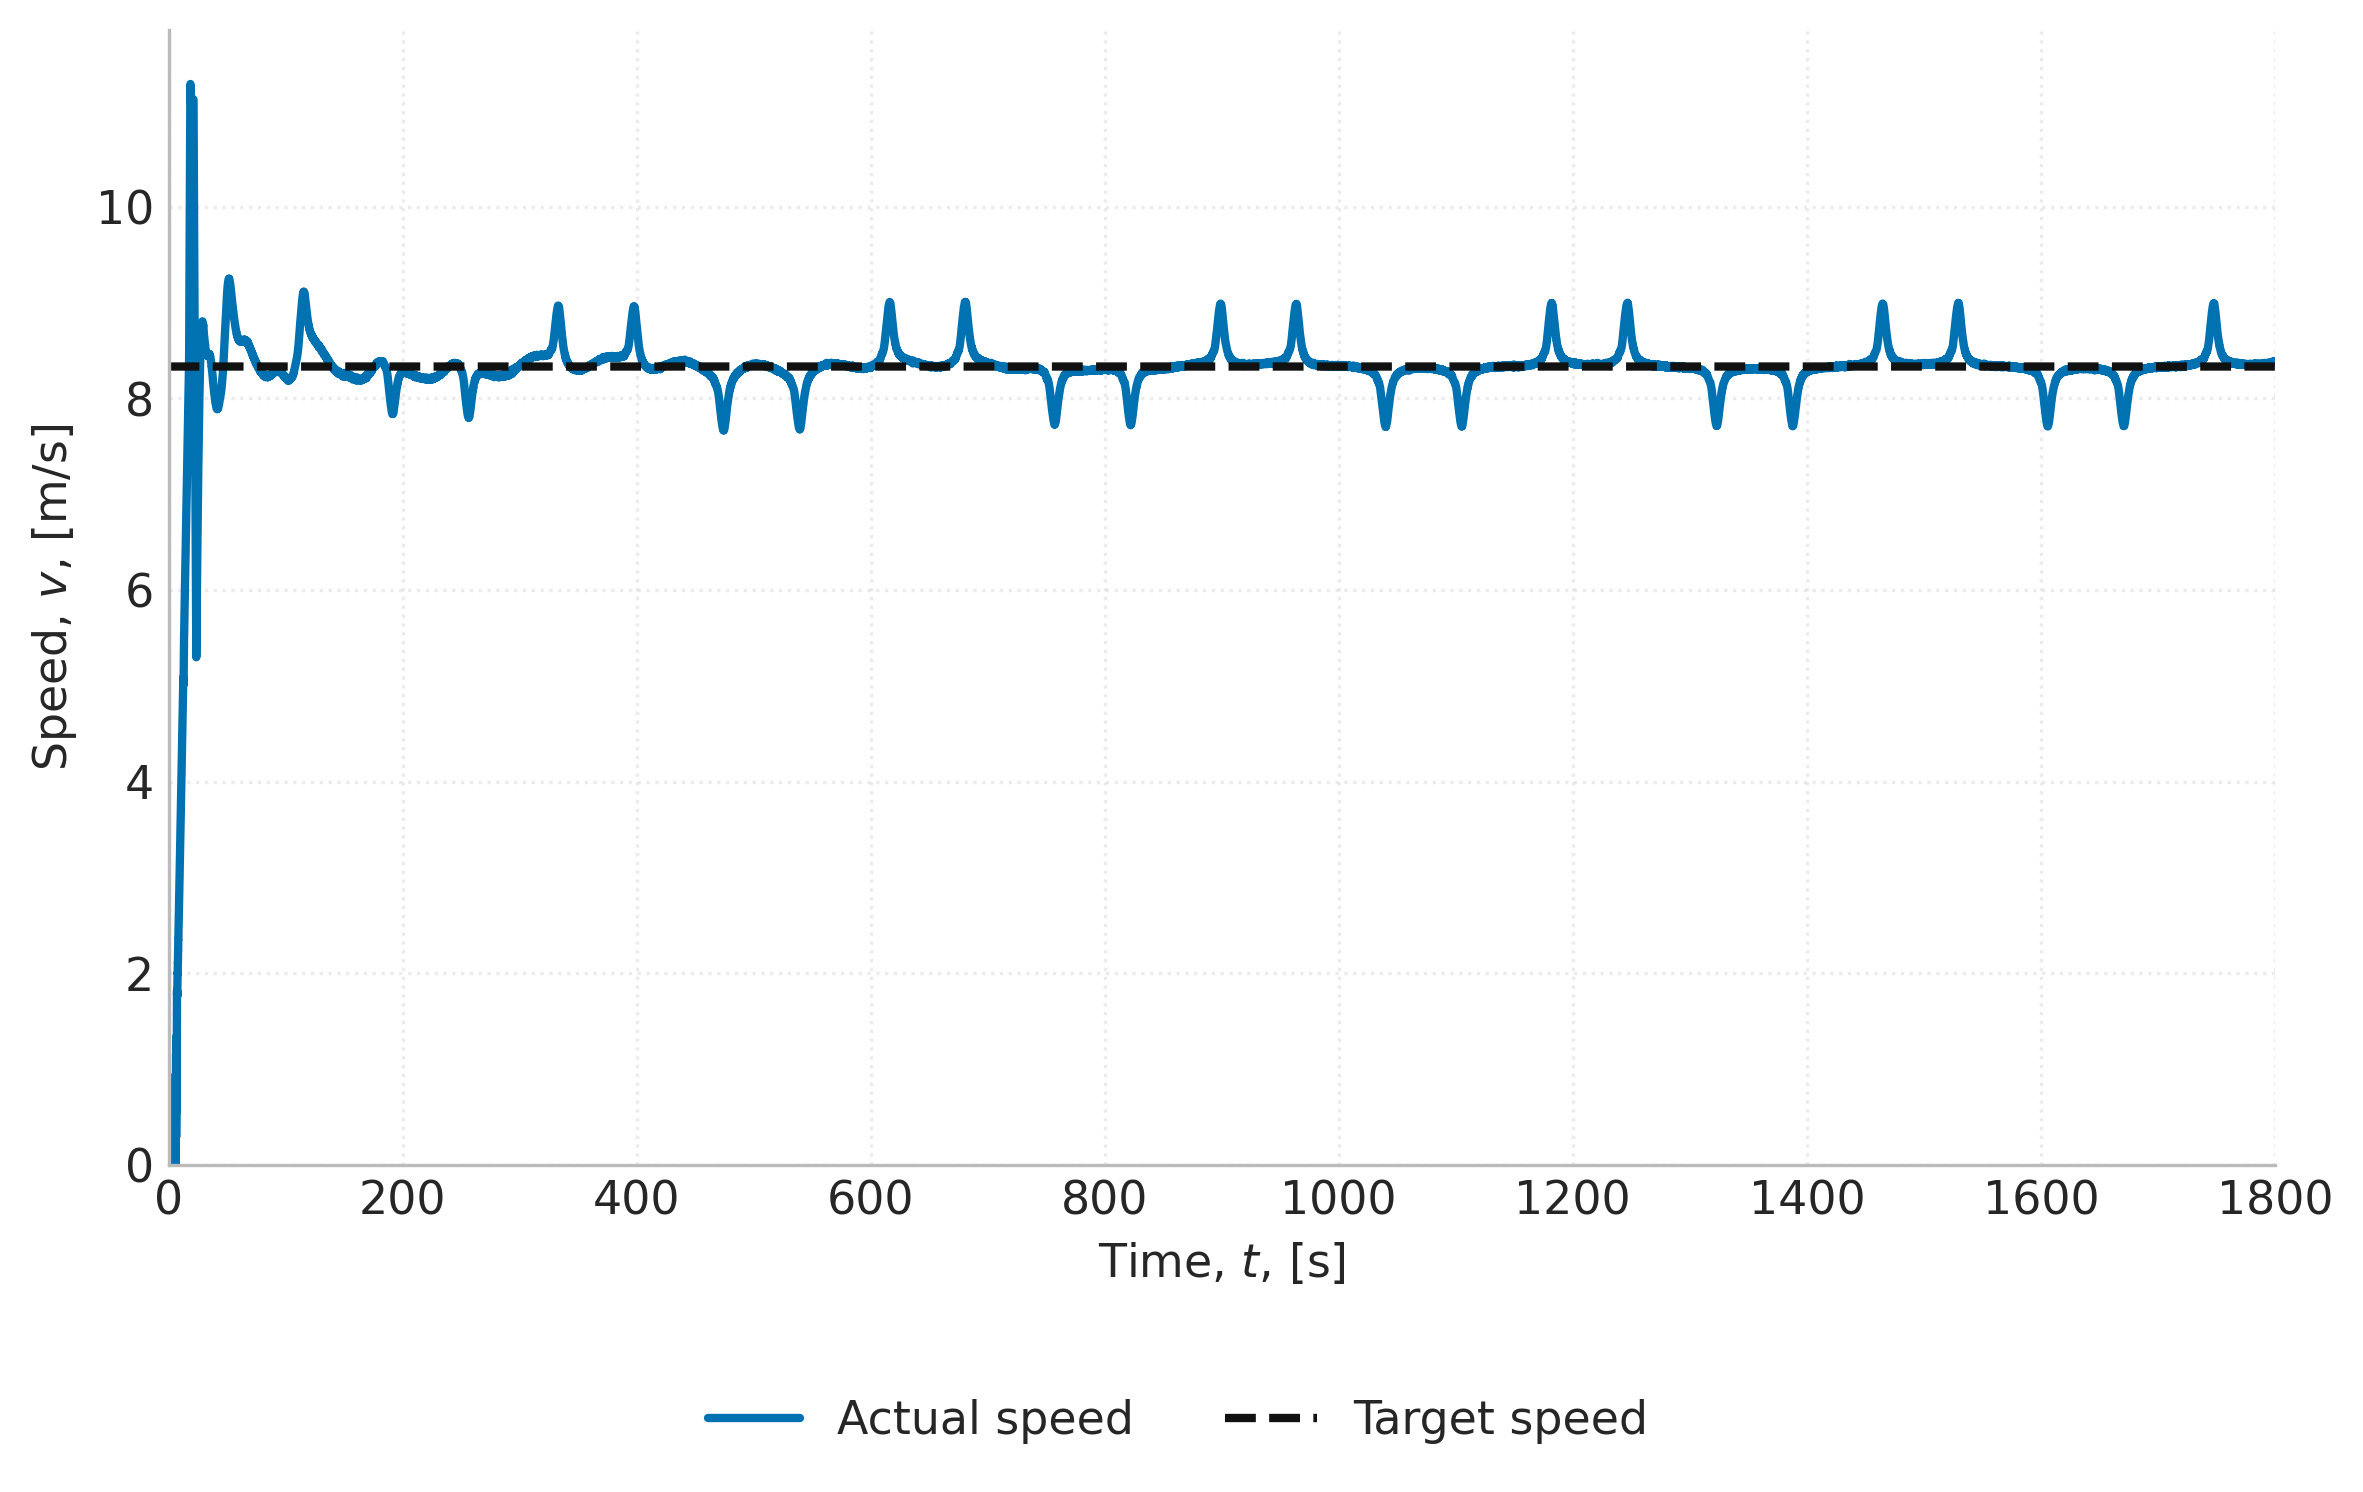
\includegraphics[width=\textwidth]{speed61.png}
        \caption{Speed Profile}
        \label{fig:speed61}
    \end{subfigure}
    \hfill
    \begin{subfigure}[b]{0.48\textwidth}
        \centering
        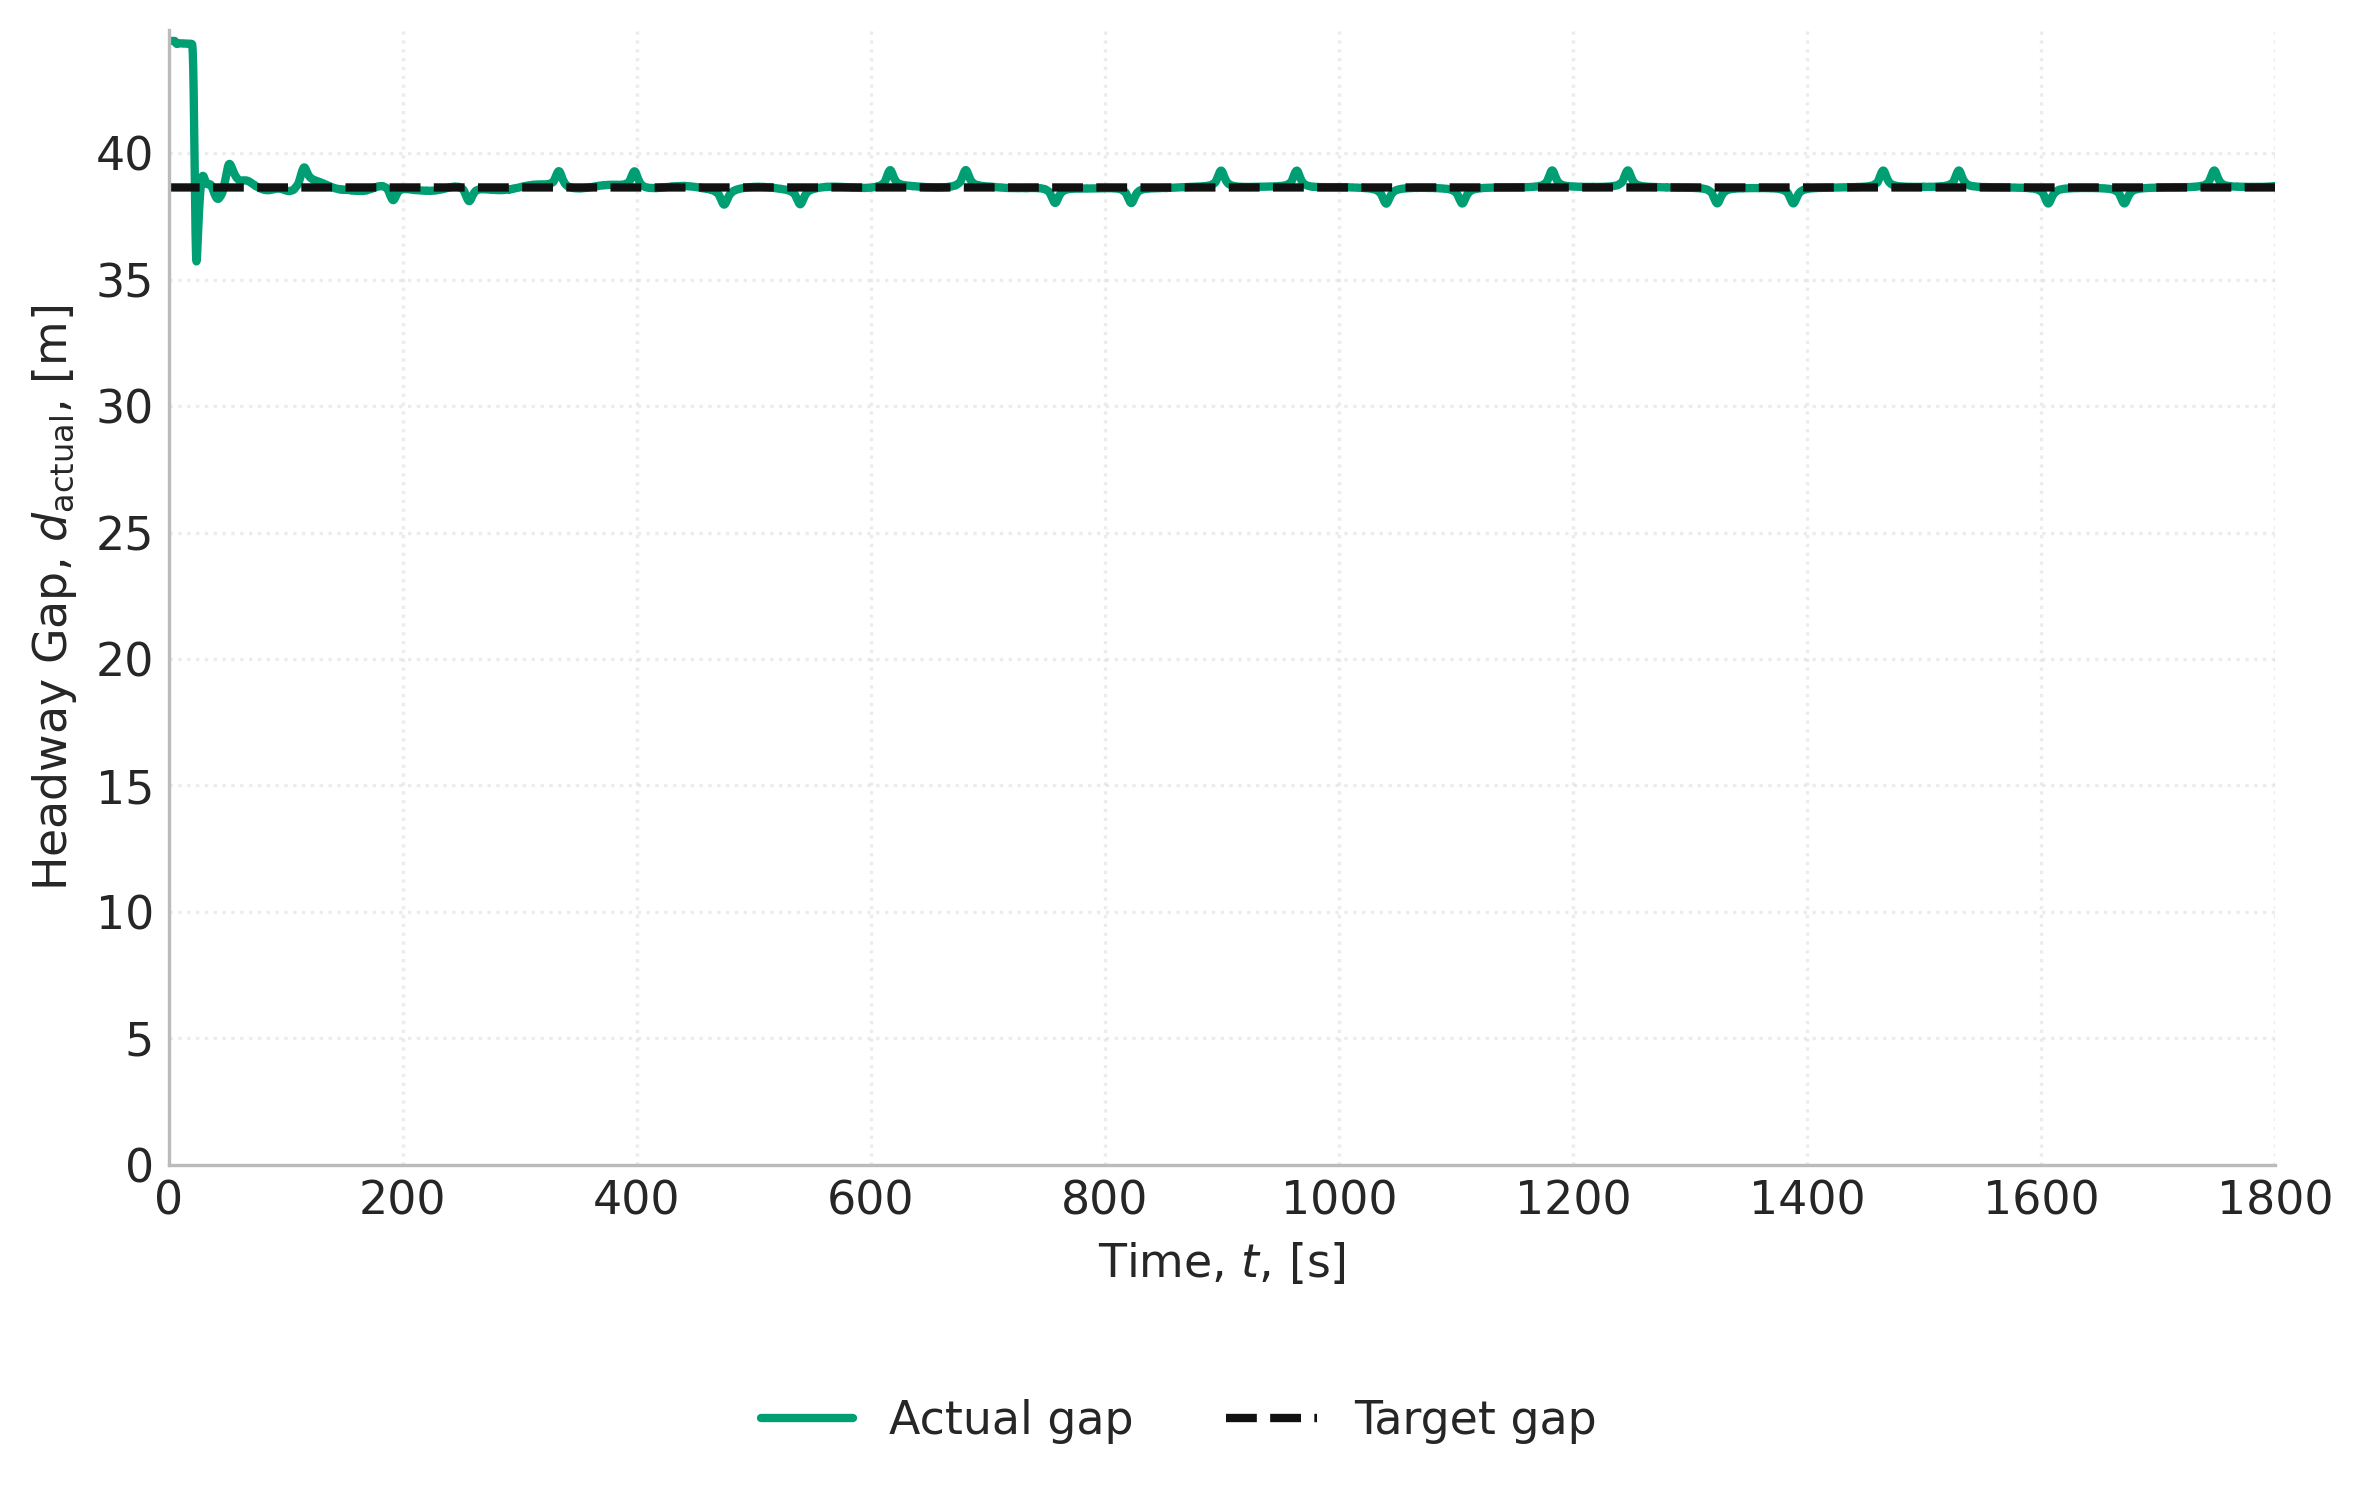
\includegraphics[width=\textwidth]{gap61.png}
        \caption{Gap Distance}
        \label{fig:gap61}
    \end{subfigure}
    
    \vspace{10pt} % Adds vertical spacing between the rows
    \begin{subfigure}[b]{0.48\textwidth}
        \centering
        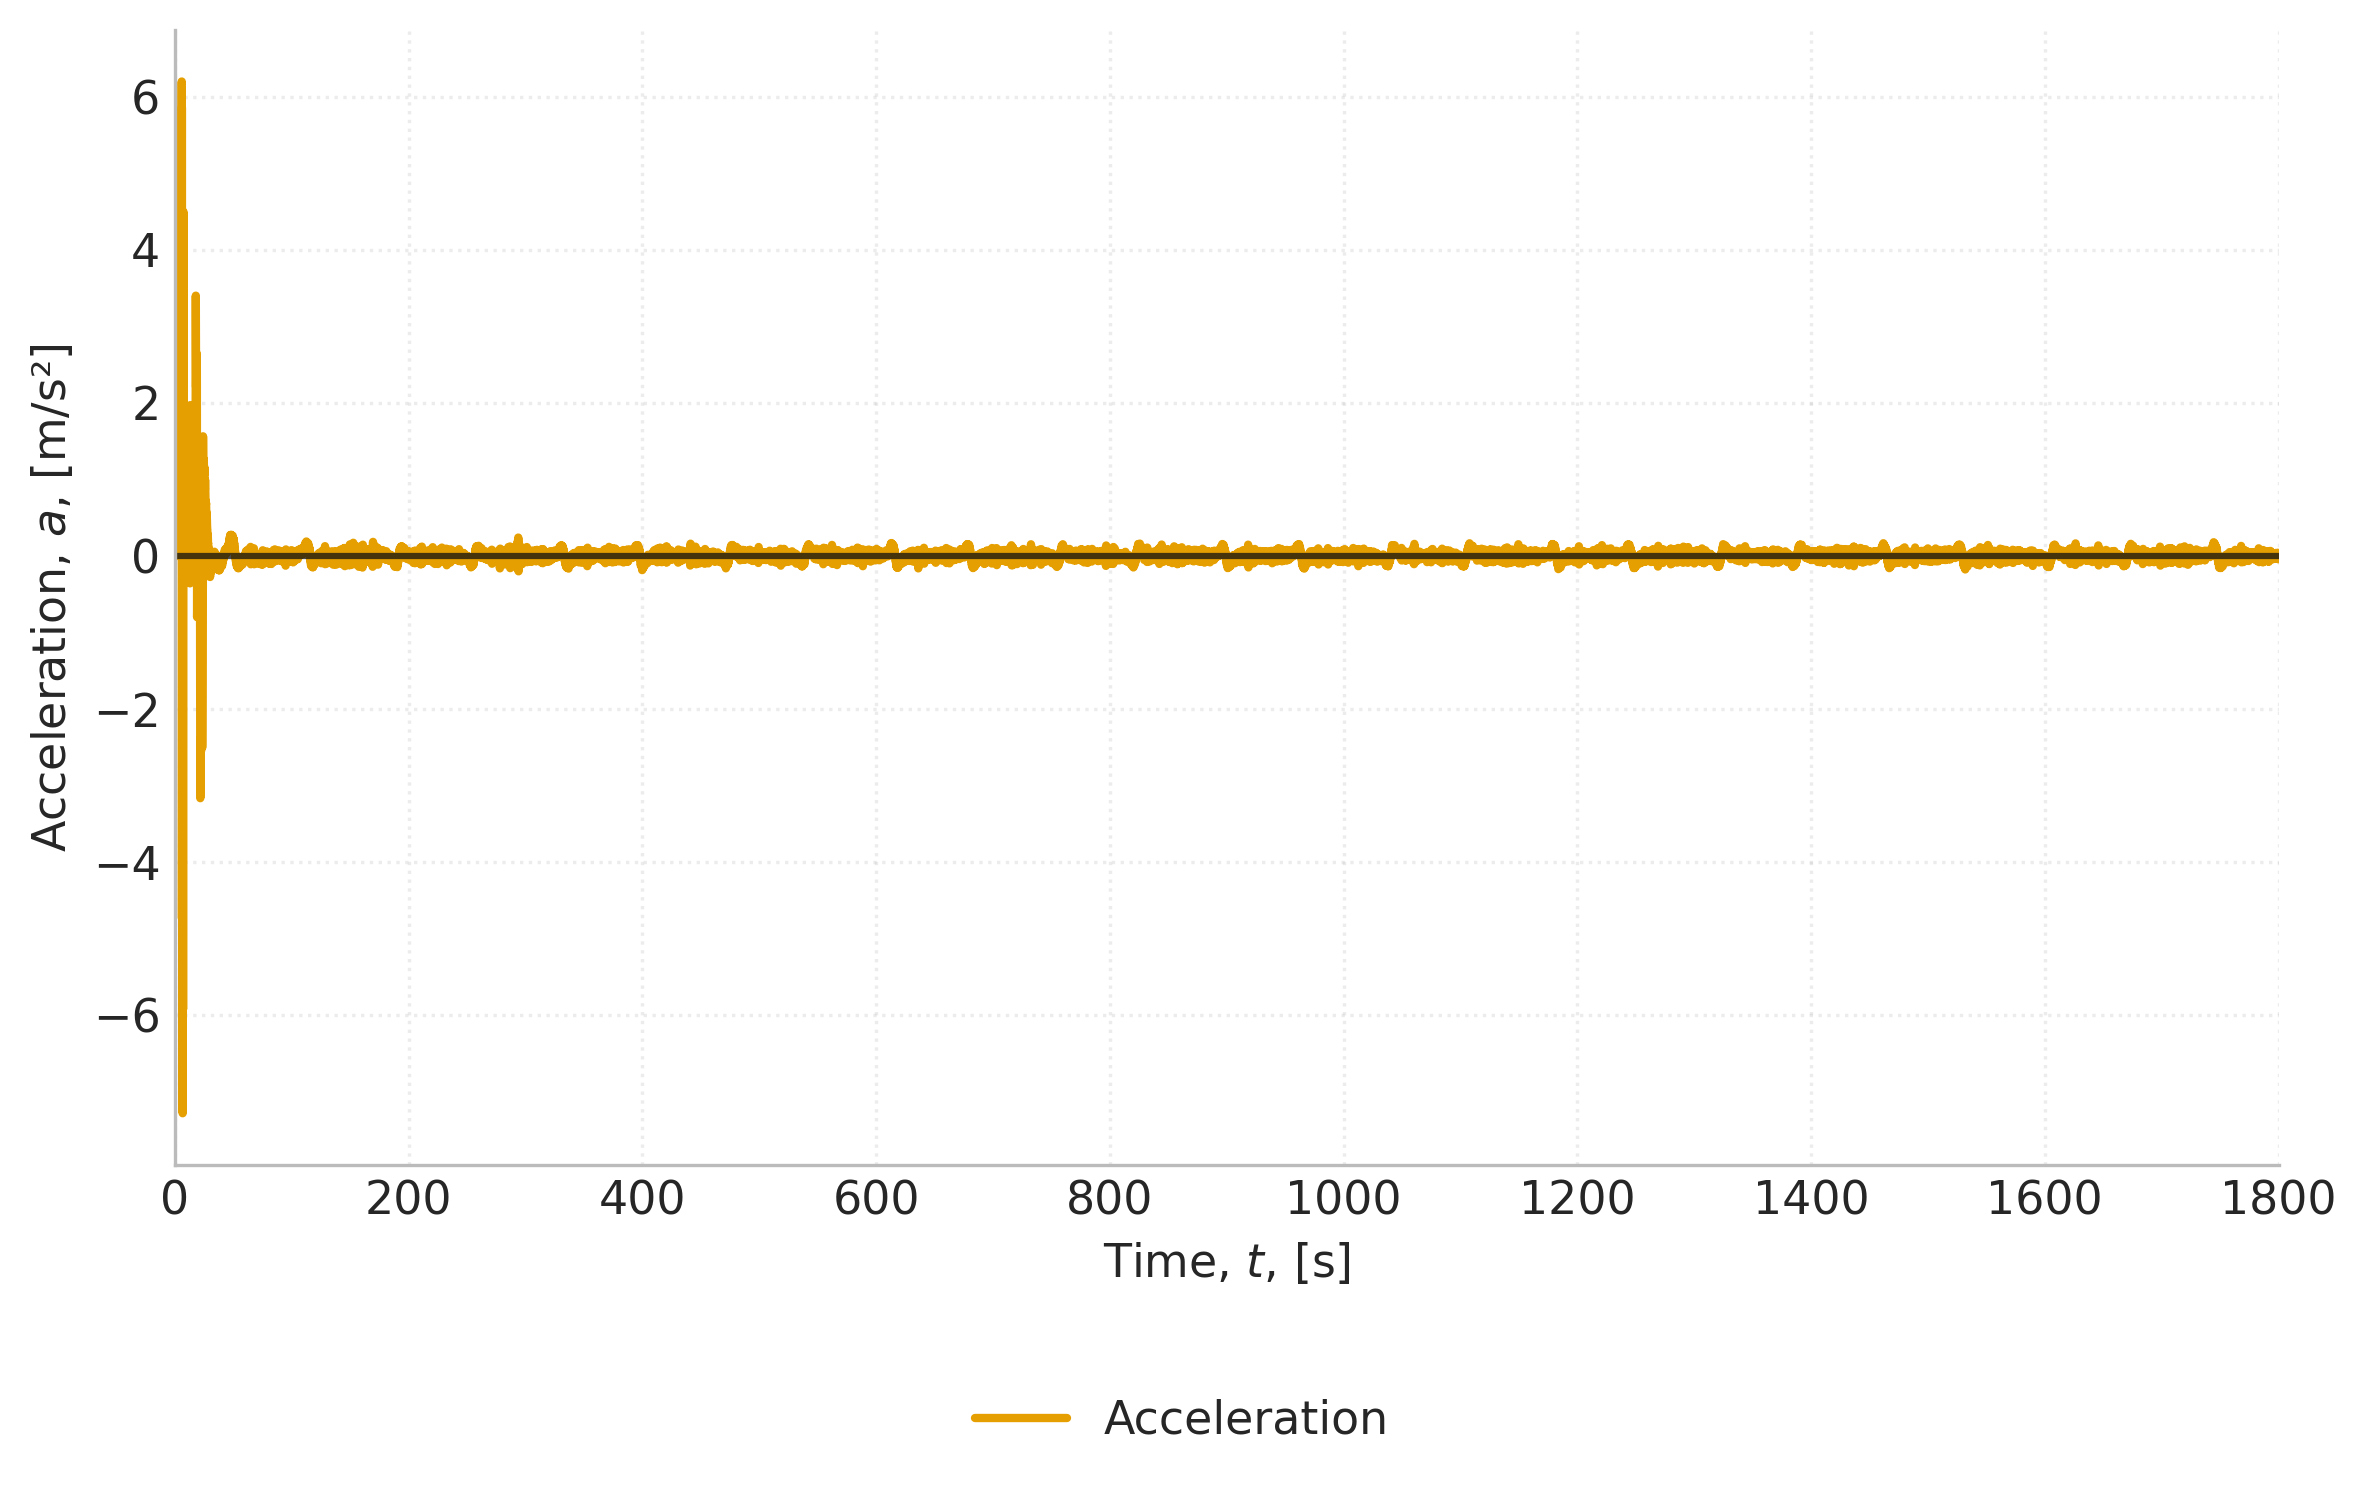
\includegraphics[width=\textwidth]{acceleration61.png}
        \caption{Acceleration Profile}
        \label{fig:accel61}
    \end{subfigure}
    \hfill
    \begin{subfigure}[b]{0.48\textwidth}
        \centering
        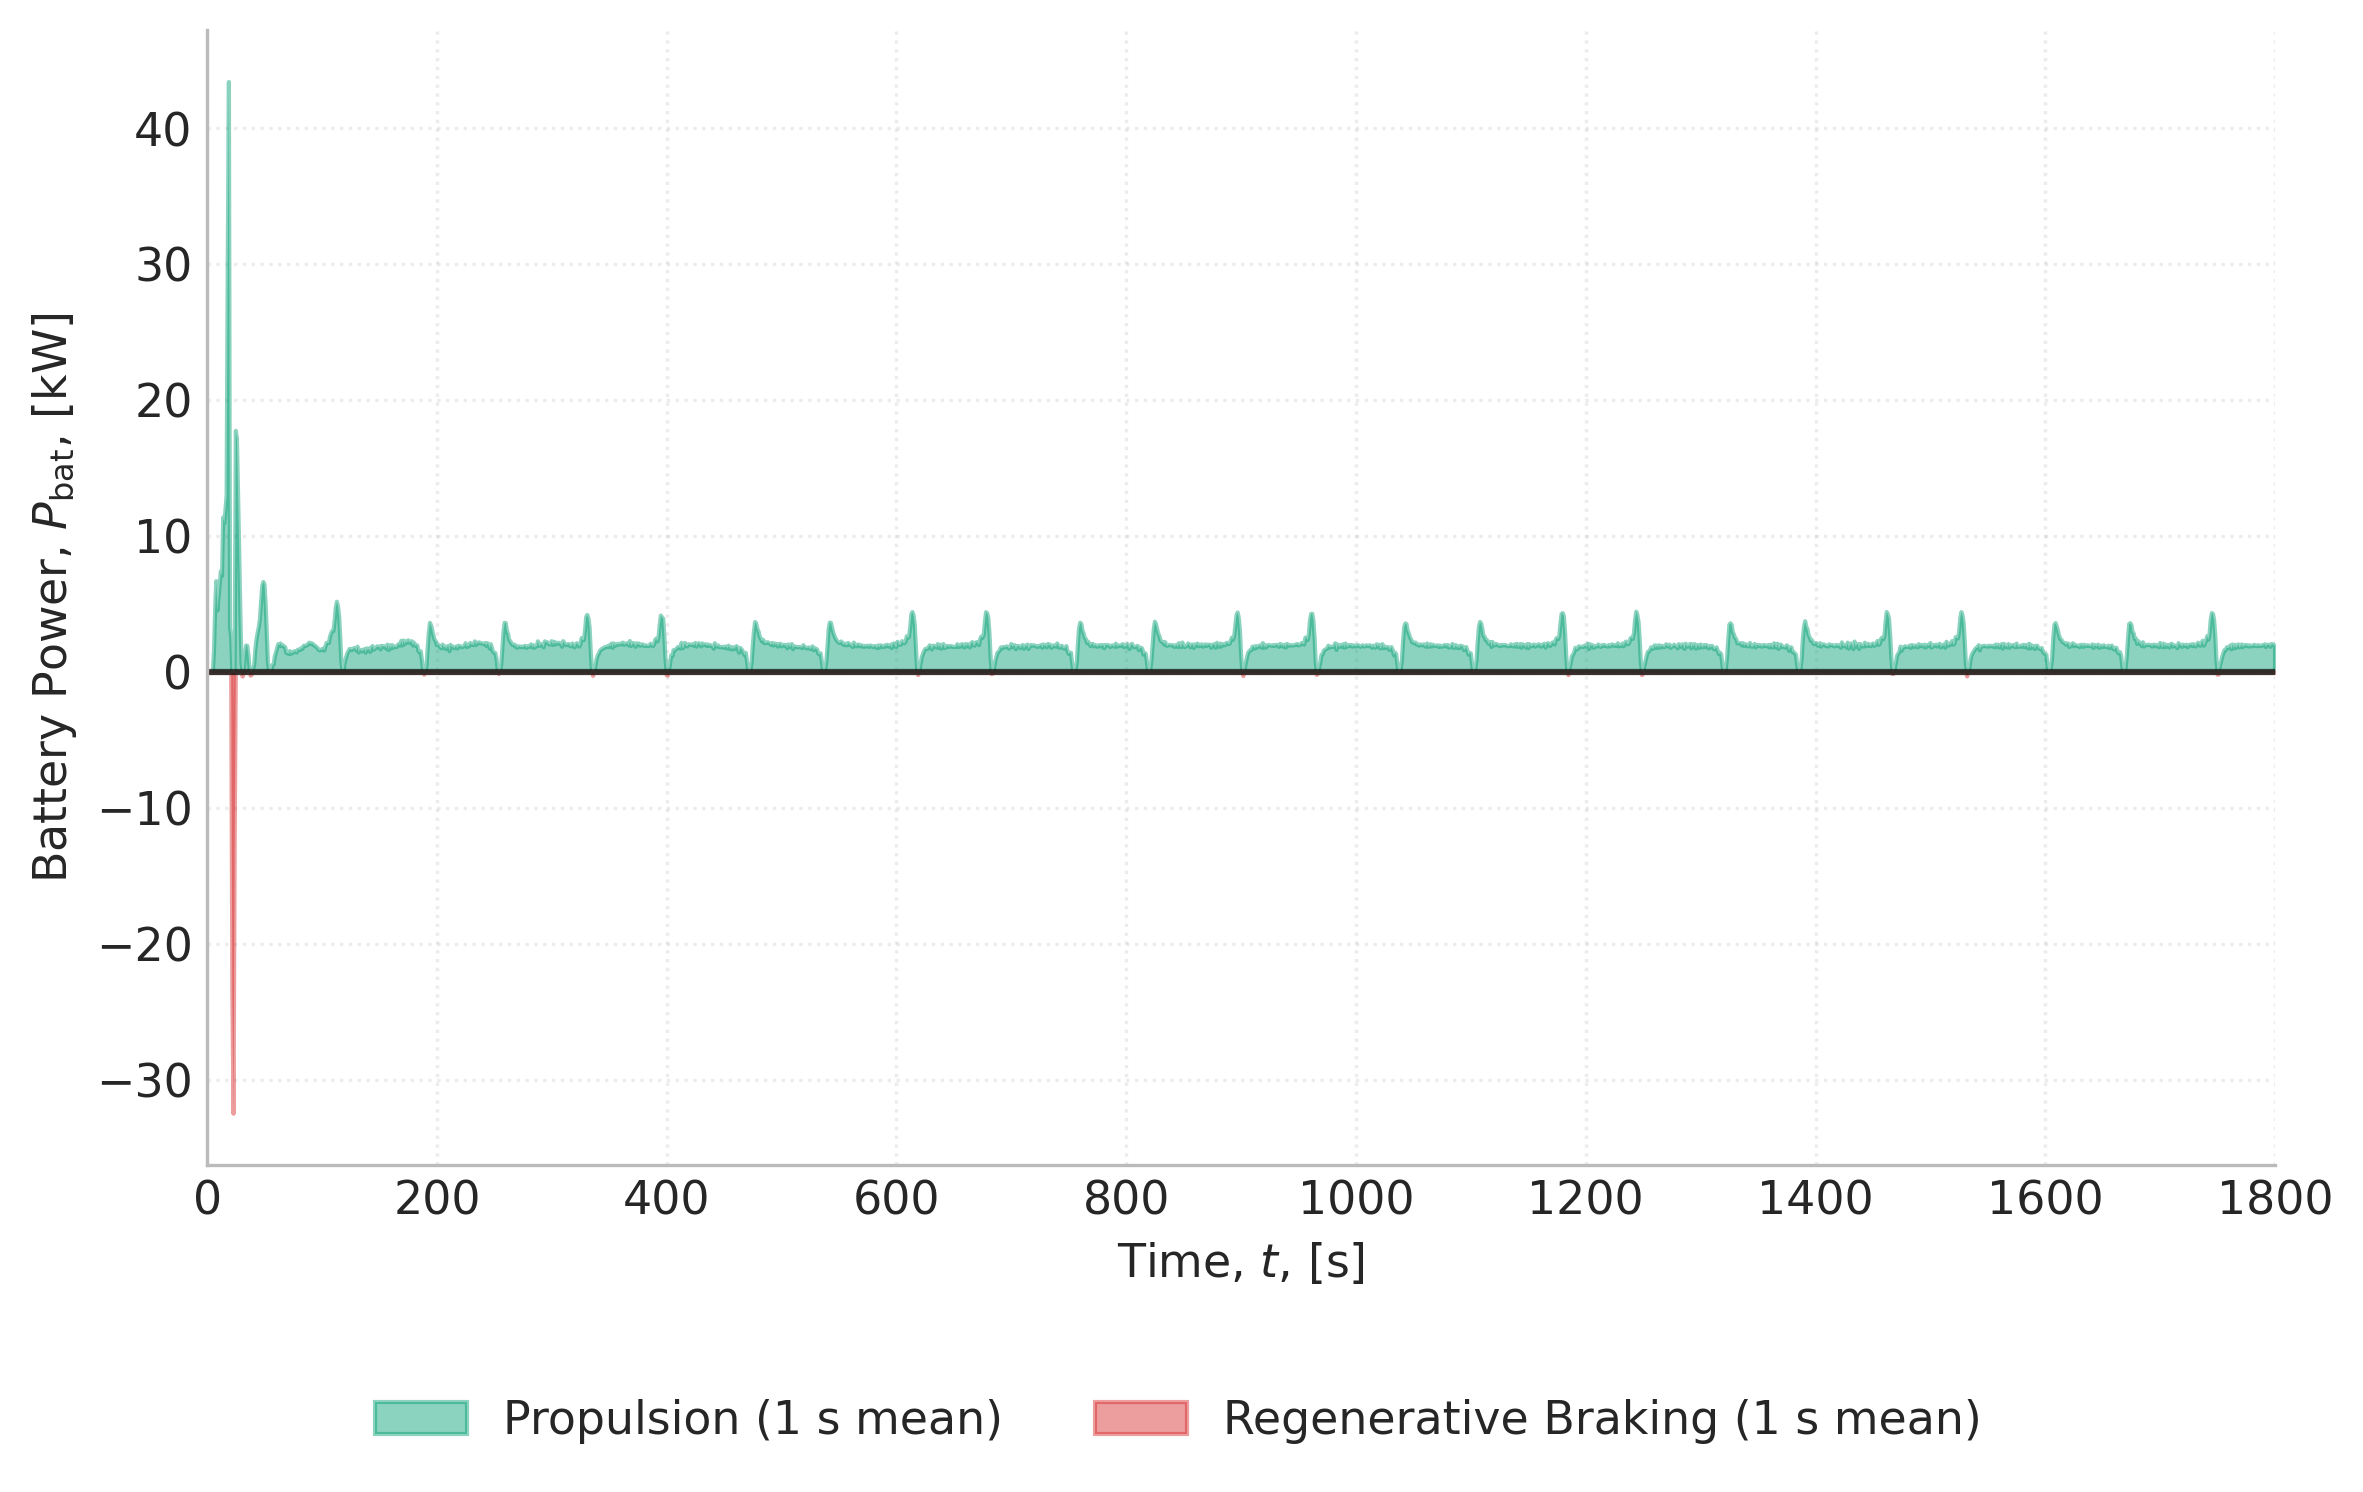
\includegraphics[width=\textwidth]{power61.png}
        \caption{Power Consumption}
        \label{fig:power61}
    \end{subfigure}
    
    \caption{Comprehensive analysis of vehicle metrics for barrier controller; showing acceleration, speed, gap distance, and power consumption for vehicle 1, run 1, and \(N=61\).}
    \label{fig:barrier}
\end{figure}

\subsubsection{FAS Controller Vehicle Behavior}
The vehicle behavior of the FAS controller is illustrated in figure~\ref{fig:fas}, showing accelerations, speed, following gap, and drive power for the same vehicle with identical conditions as described in the previous section.
\\\\
The speed profile, figure~\ref{fig:speed61fas}, shows clear stop-and-go behavior, which can be seen by the actual speed reaching 0, and then increasing again to approximately 11 m/s. The figure also displays that the vehicle often cruises below the target speed at approximately 6 m/s. All in all, it can be seen that the vehicle never cruises at target speed, but rather alters between a complete stop, cruising above the target speed due to large headway gaps after stopping at the traffic light, or cruising below target speed during driving within a queue that has not yet stopped. 
\\\\
The following gap, figure~\ref{fig:gap61fas}, shows that the gap never settles around the target gap, which is in line with the speed profile. The actual gap is either around 6 to 8 m during queuing, or it is above target when the vehicle in front accelerates quickly after a red light due to a large gap error to its predecessor, or it is below target during driving in a queue that has not yet reached a stop. All in all, the FAS controller does not maintain the target spacing, which is expected since vehicles are stopped at the traffic light.
\\\\
The acceleration, section~\ref{fig:acceleration61fas}, also shows stop-and-go behavior, characterized by large accelerations and decelerations. With respect to the latter, it can be seen that the vehicle decelerates at -7.5 \(m/s^2\), which is far more aggressive than a comfortable deceleration of 2.5 \(m/s^2\) \parencite{carlowitz2026balancing}. 
\\\\
Drive power, figure~\ref{fig:power61fas}, illustrates propulsion peaks during acceleration peaks, and regenerative braking peaks during deceleration peaks.  
\\\\
In general, the FAS controller exhibits erratic behavior. Instead of cruising smoothly at all targets, the vehicle shows clear stop-and-go behavior, resulting in deviation from both target gap and target speed, large accelerations and decelerations, and switching between propulsion and regenerative braking. 




\begin{figure}[H]
    \centering
    \begin{subfigure}[b]{0.48\textwidth}
        \centering
        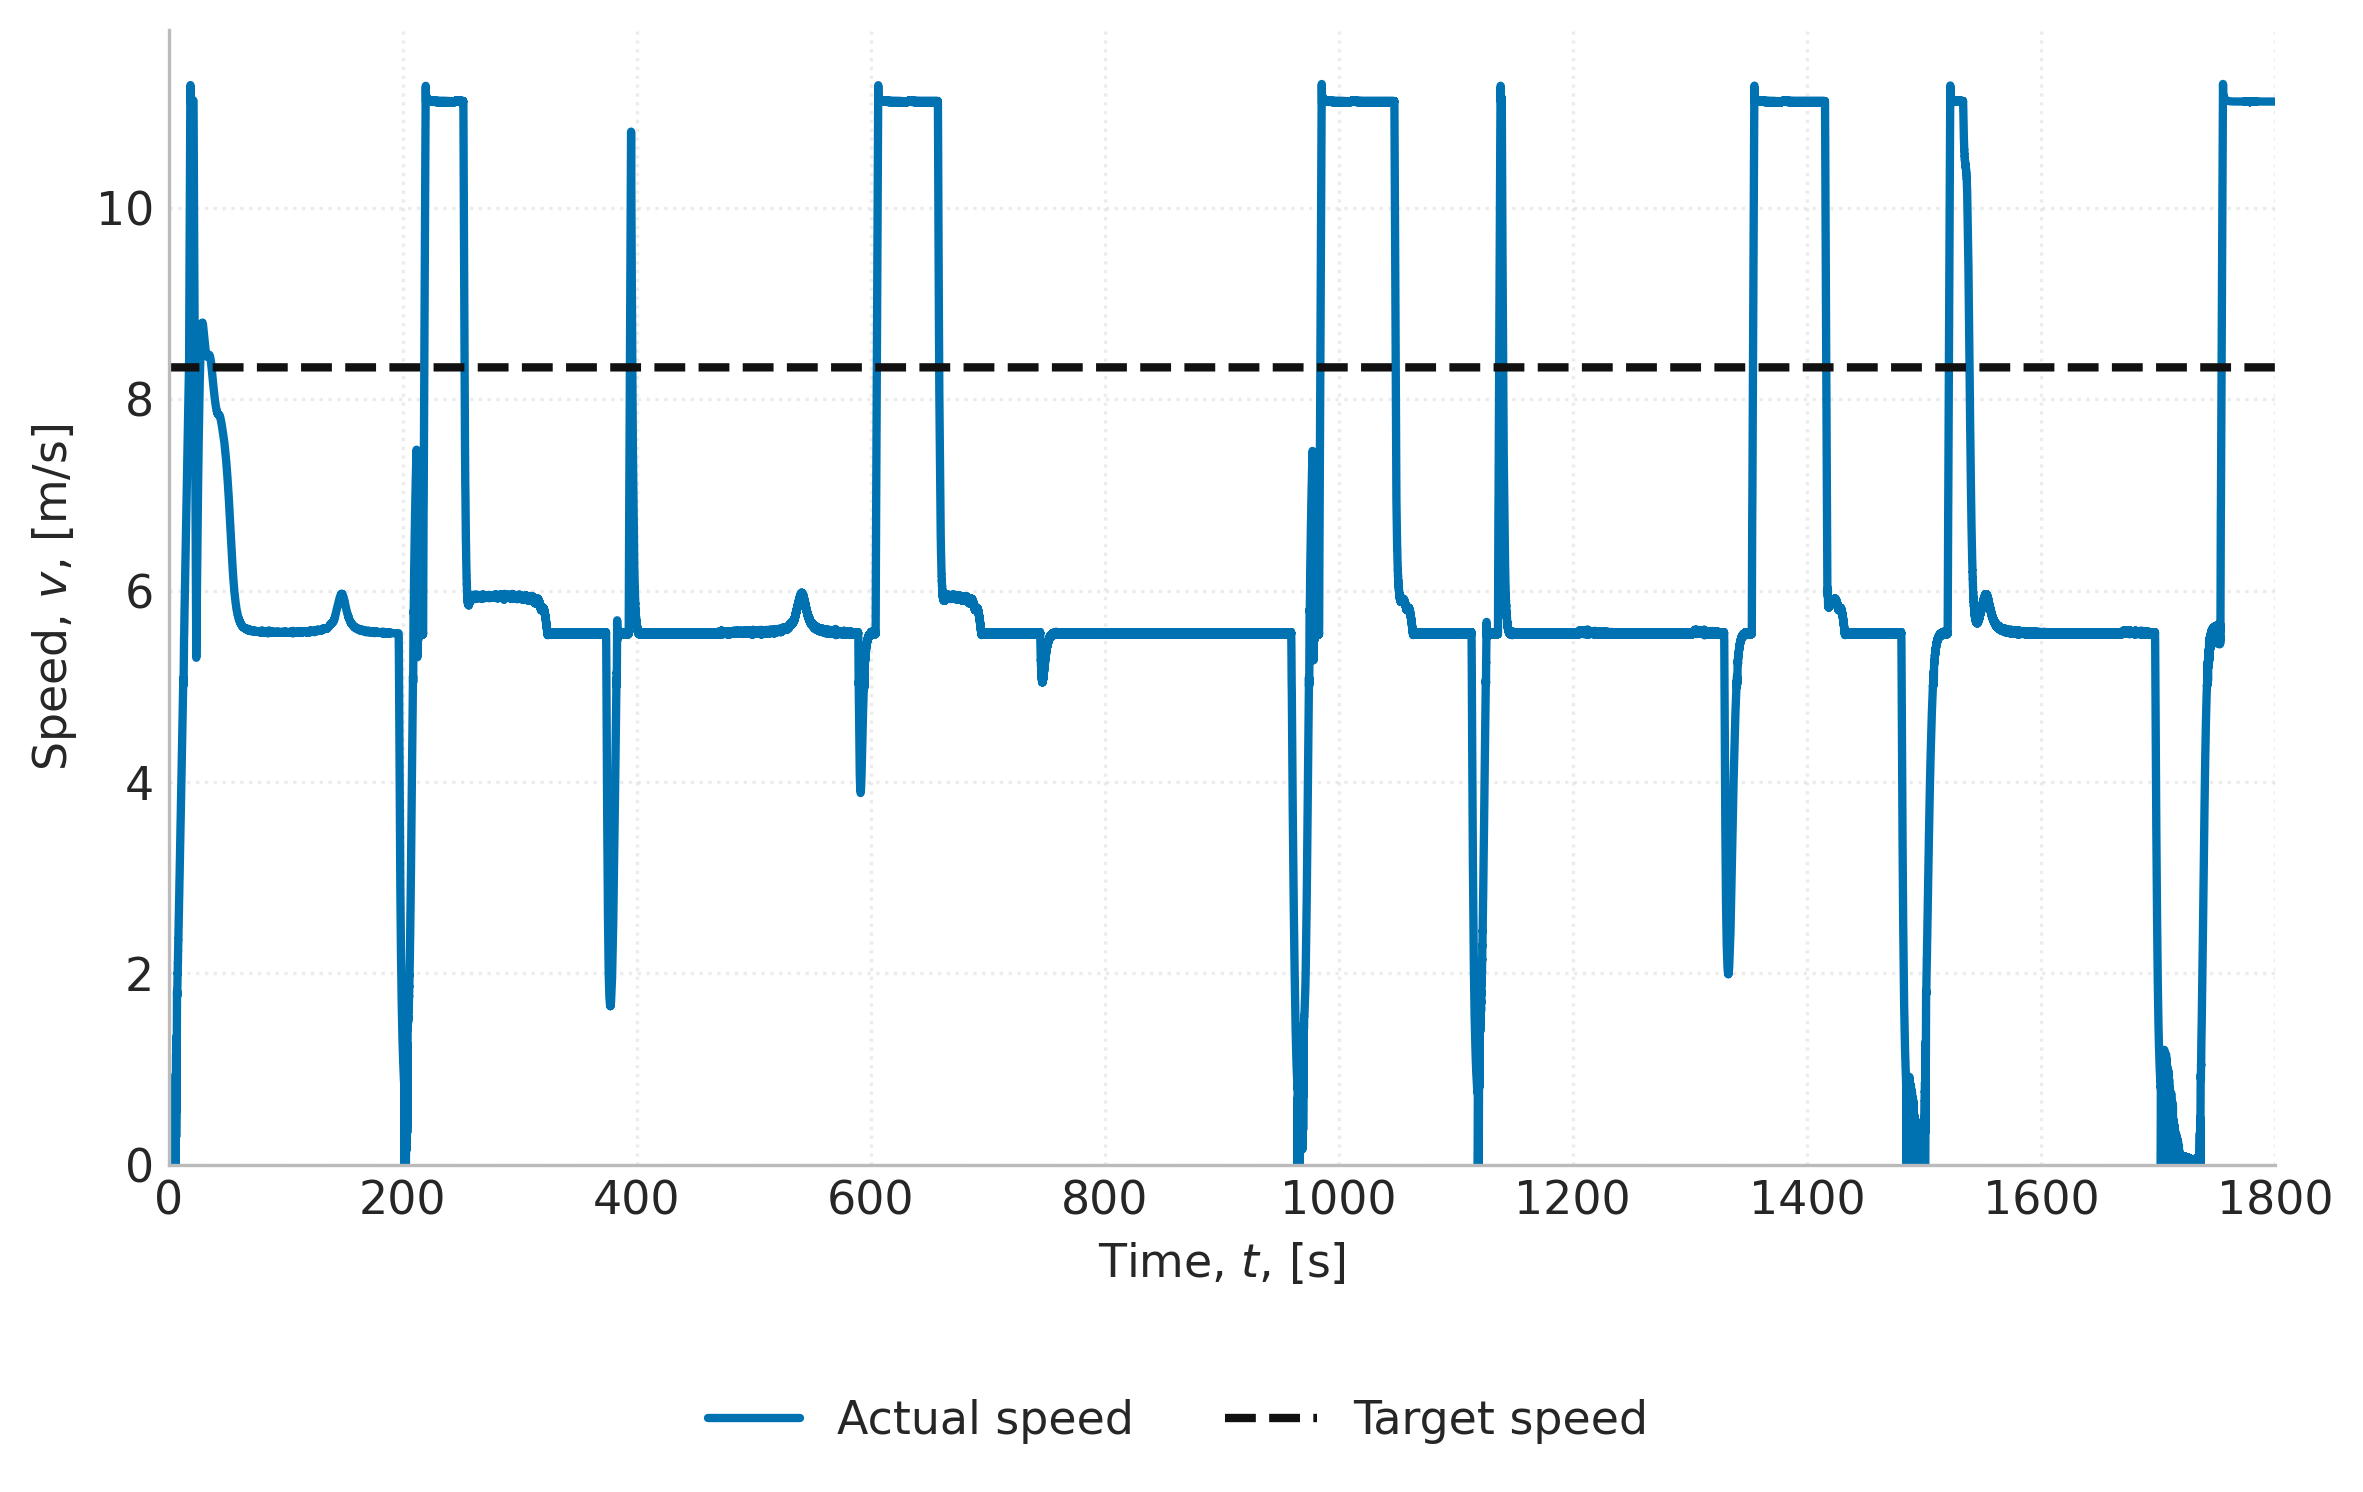
\includegraphics[width=\textwidth]{speed61fas.png}
        \caption{Speed Profile}
        \label{fig:speed61fas}
    \end{subfigure}
    \hfill
    \begin{subfigure}[b]{0.48\textwidth}
        \centering
        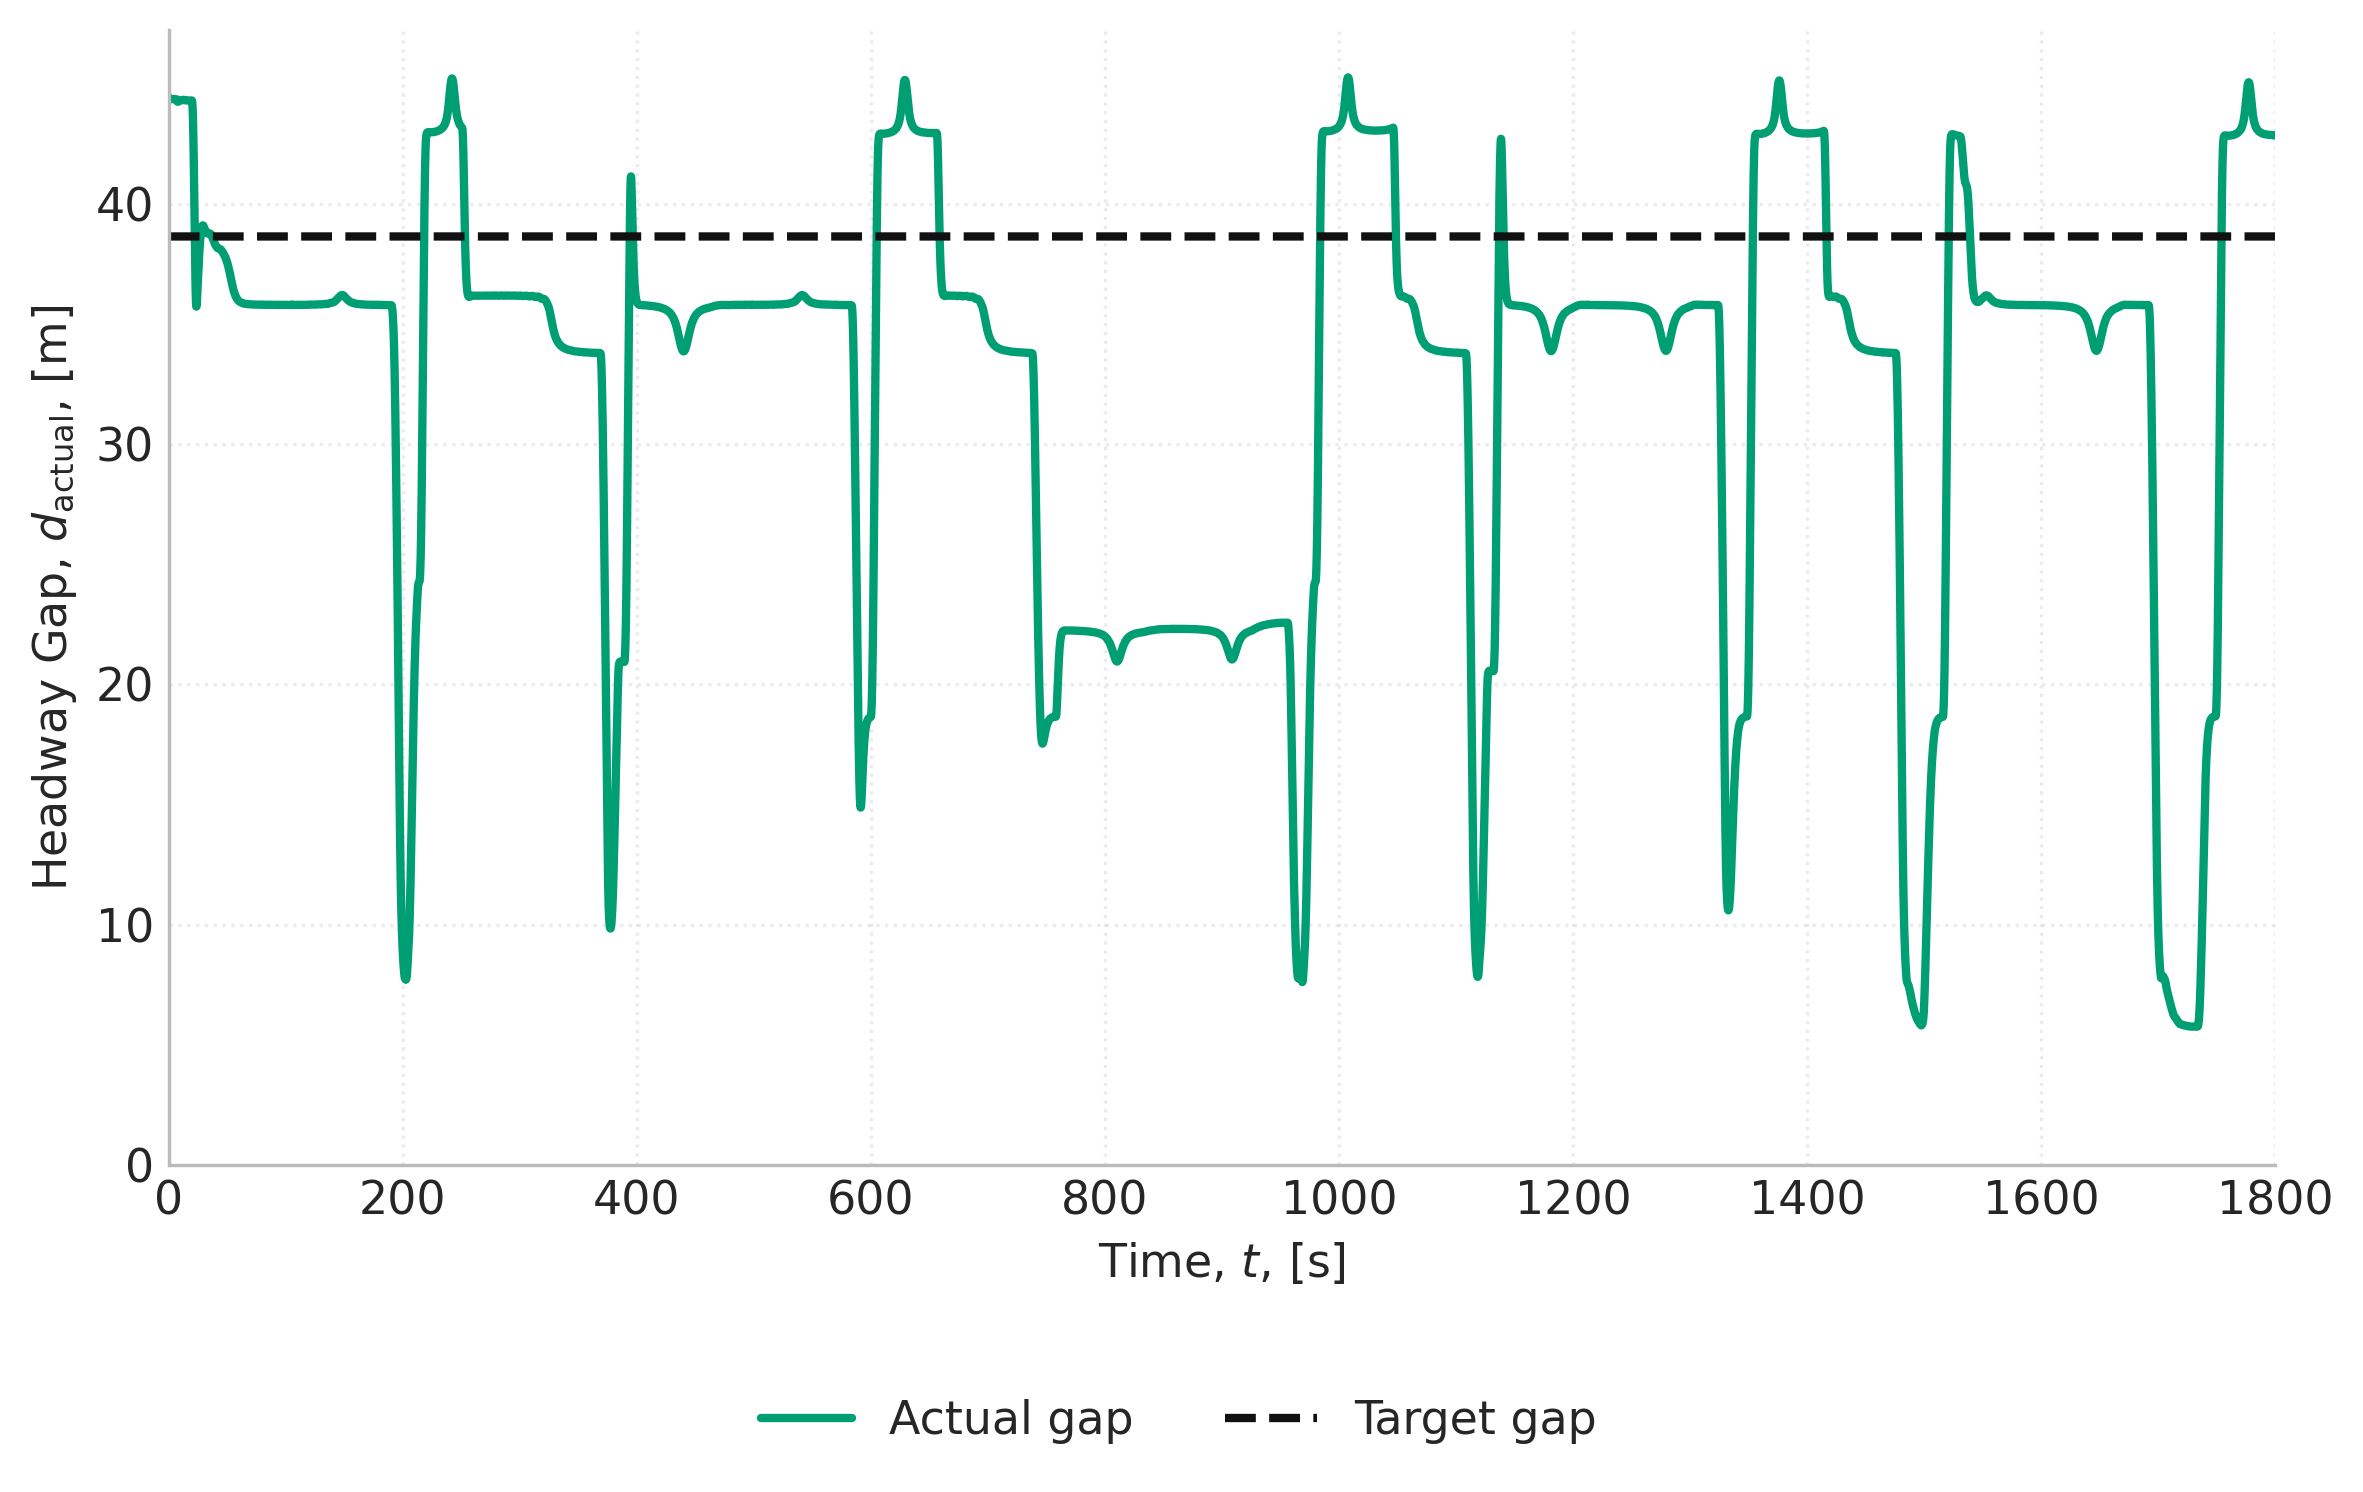
\includegraphics[width=\textwidth]{gap61fas.png}
        \caption{Gap Distance}
        \label{fig:gap61fas}
    \end{subfigure}
    
    \vspace{10pt} % Adds vertical spacing between the rows
     \begin{subfigure}[b]{0.48\textwidth}
        \centering
        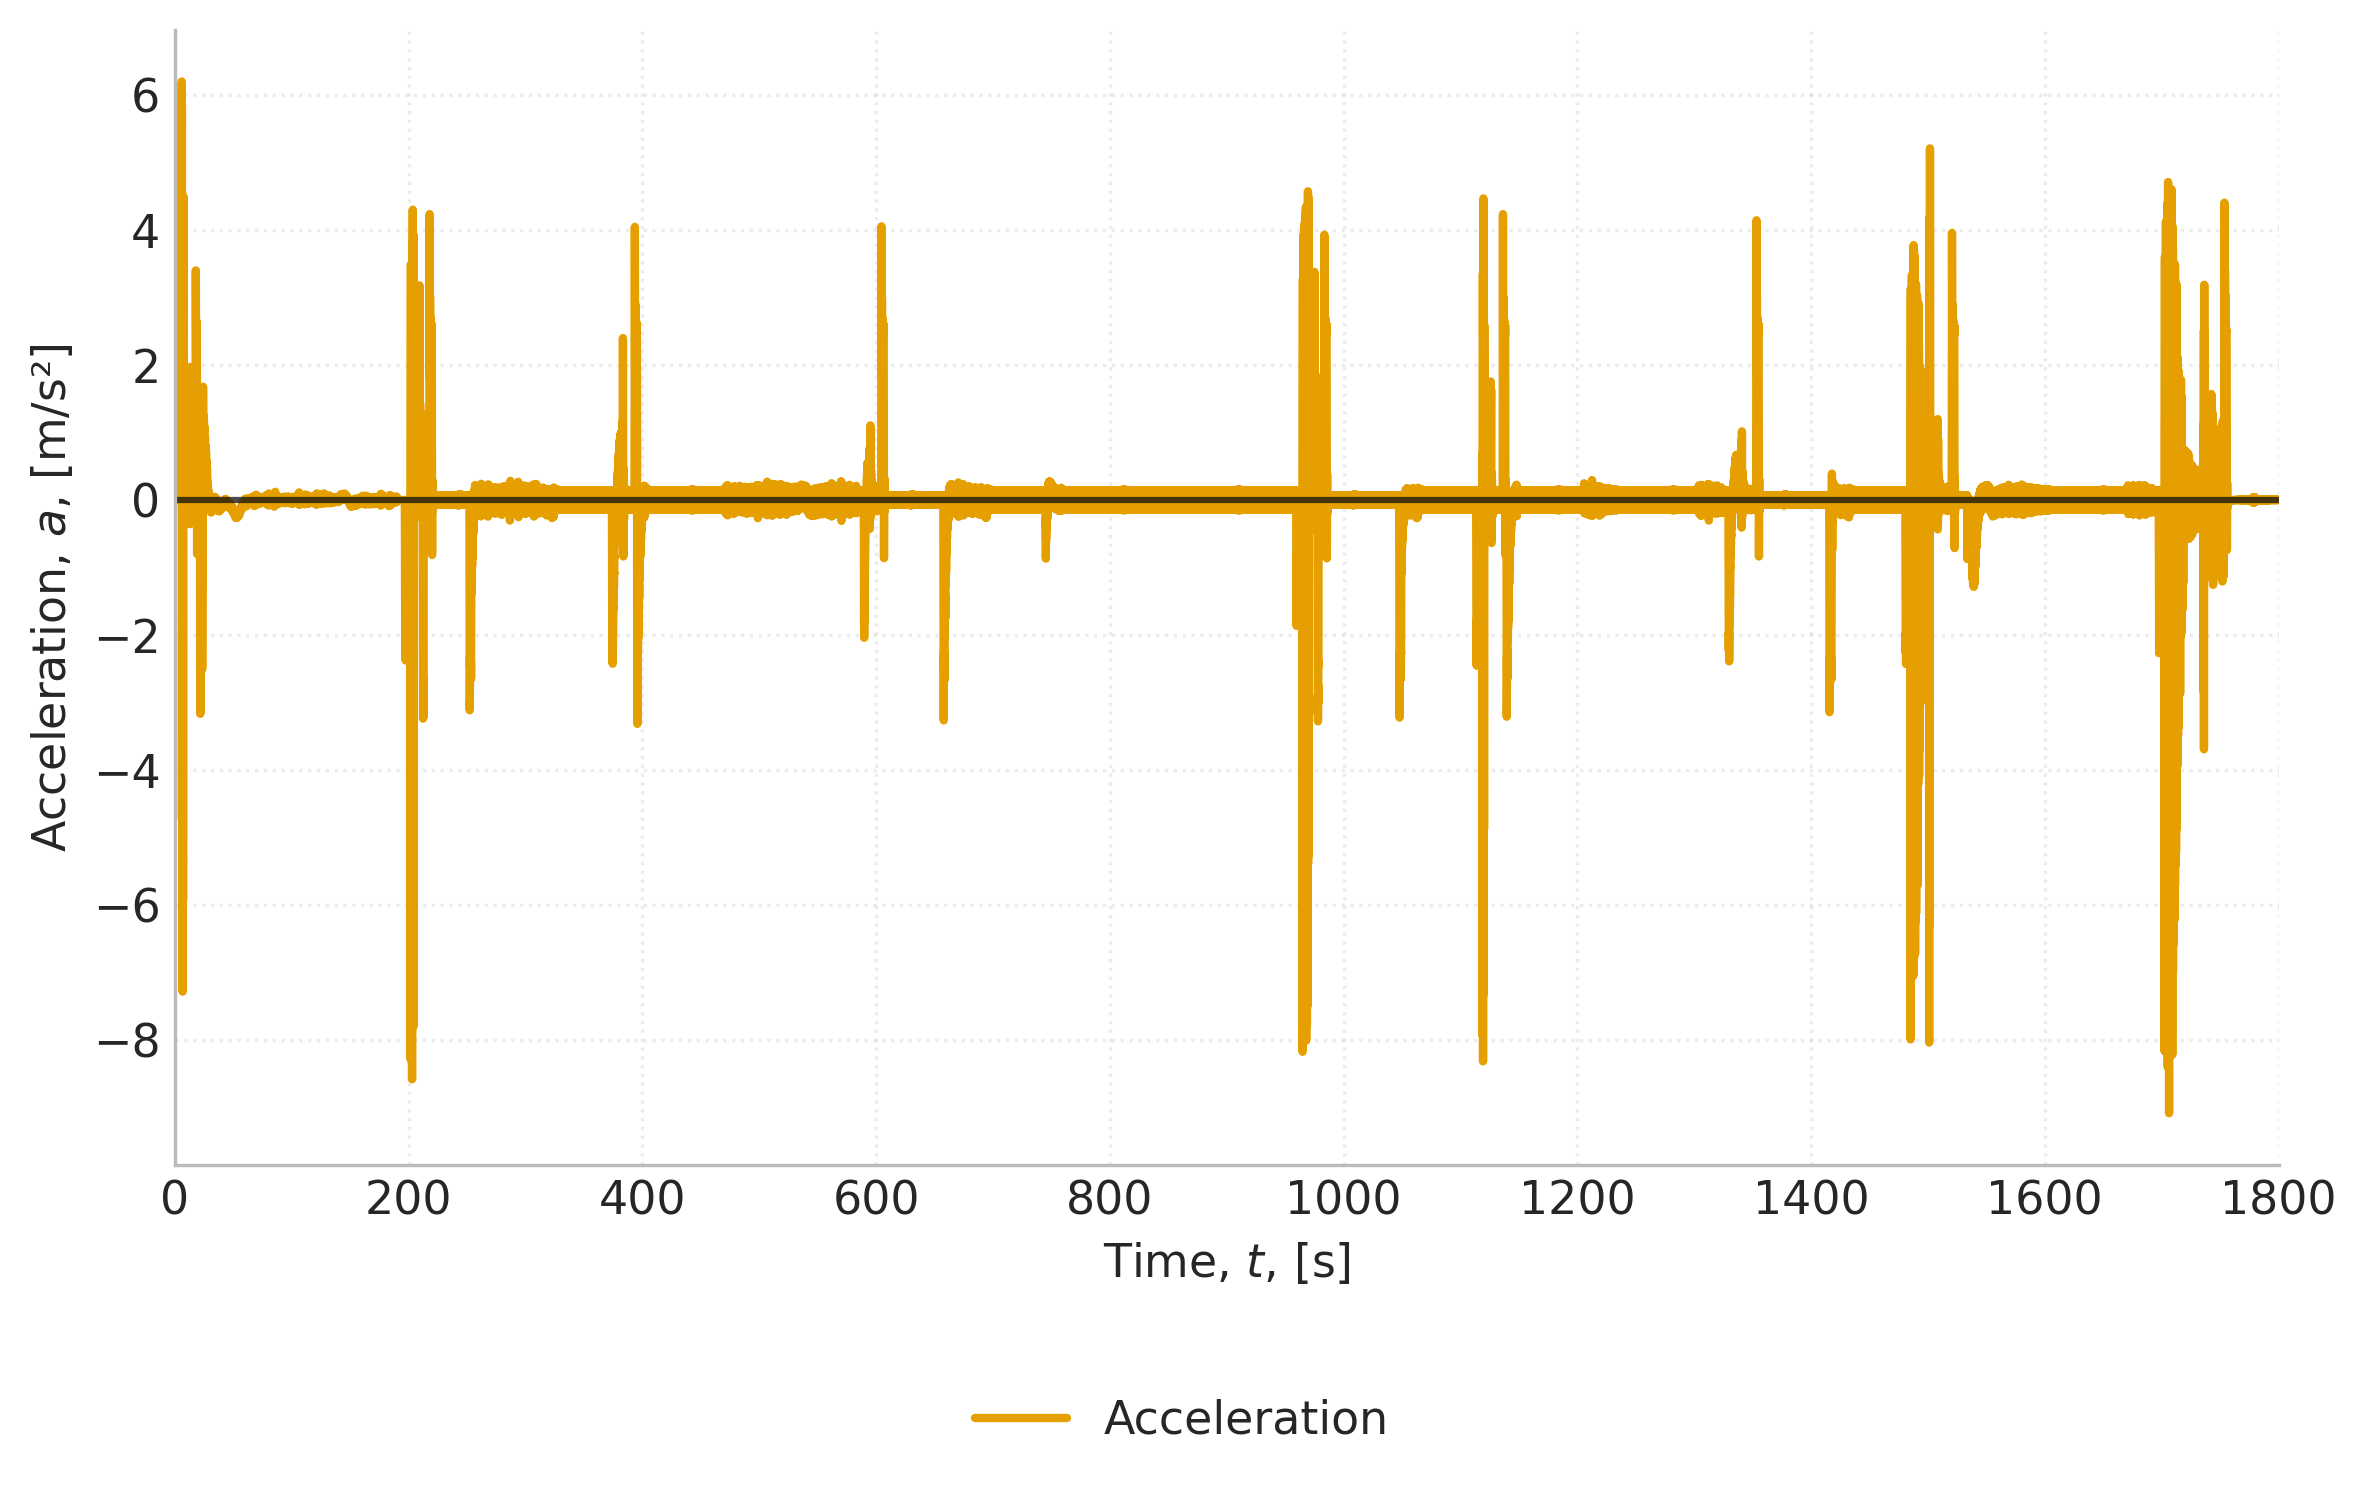
\includegraphics[width=\textwidth]{acceleration61fas.png}
        \caption{Acceleration Profile}
        \label{fig:acceleration61fas}
    \end{subfigure}
    \hfill
    \begin{subfigure}[b]{0.48\textwidth}
        \centering
        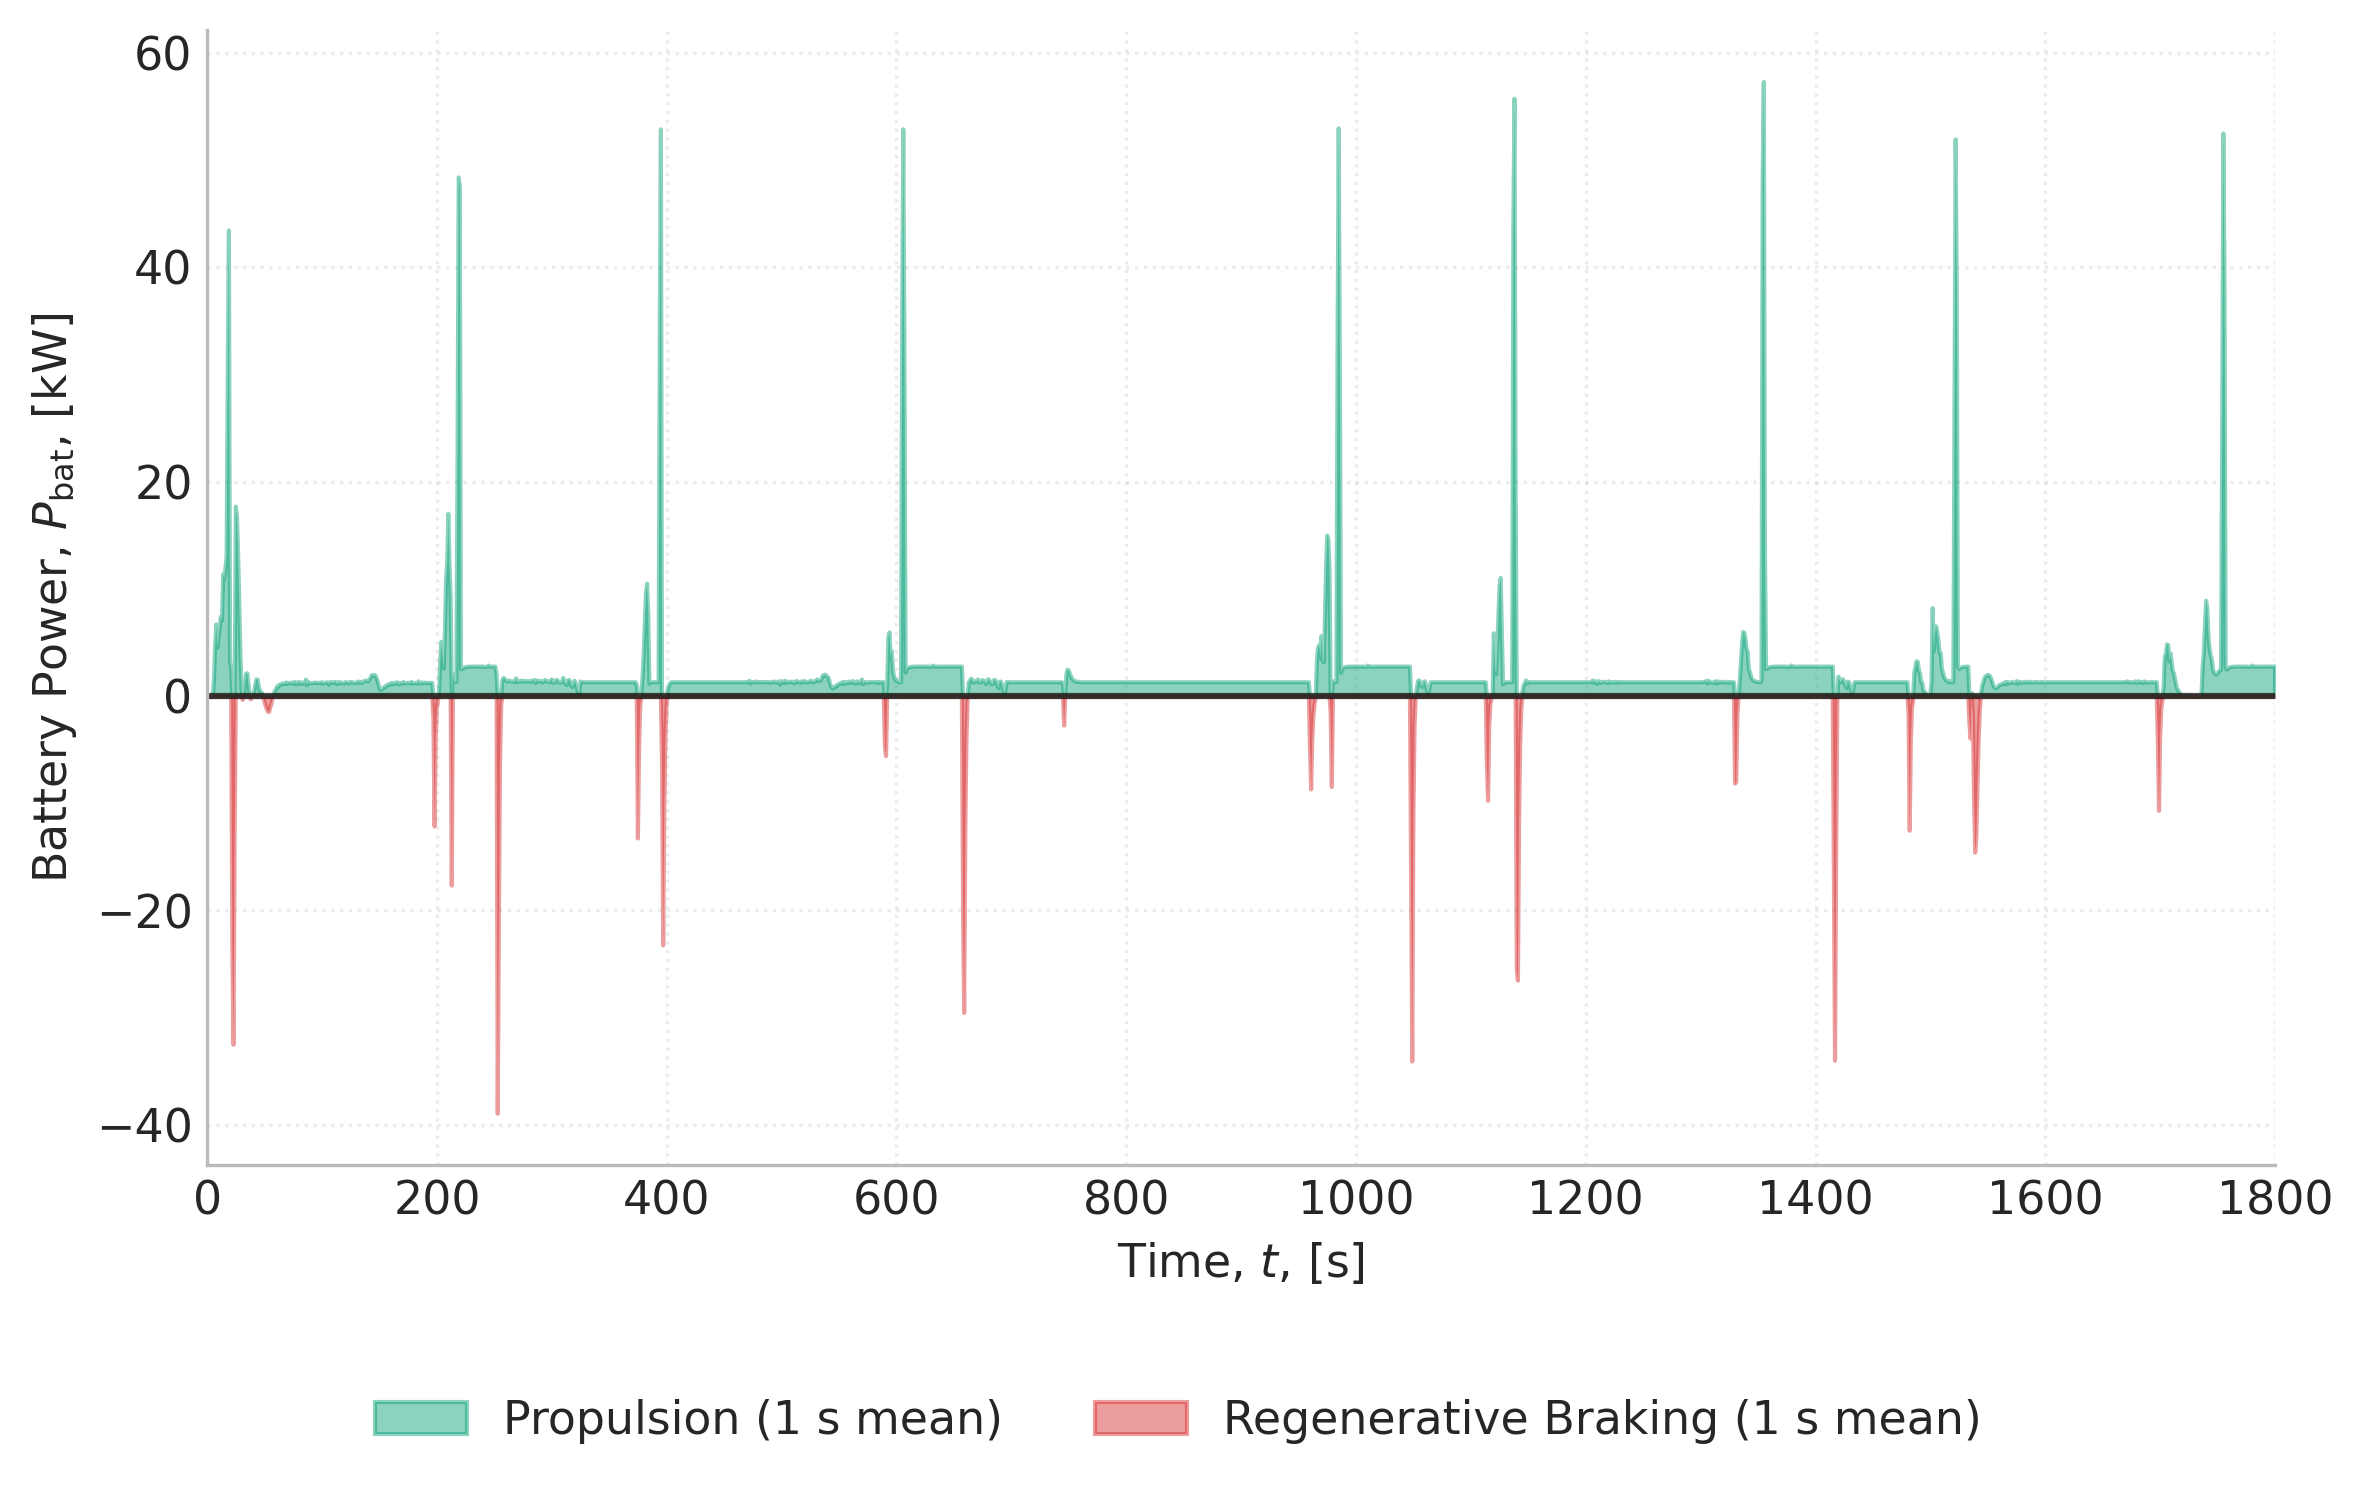
\includegraphics[width=\textwidth]{power61fas.png}
        \caption{Power Consumption}
        \label{fig:power61fas}
    \end{subfigure}
    
    \caption{Comprehensive analysis of vehicle metrics for FAS controller; showing acceleration, speed, gap distance, and power profiles for vehicle 1, run 1, and \(N=61\).}
    \label{fig:fas}
\end{figure}

\subsection{Barrier Controller Performance}
The performance of the barrier controller is verified, in terms of activations across the various vehicle counts. Figure~\ref{fig:firings-per-demand}, shows a box-plot of the number of barrier controller activations per batch. The figure highlights, that the barrier activates more often at a higher vehicle density. At \(N=51\) vehicles, the barrier never activates across all runs. Similar behavior is seen at \(N=61\), where the barrier fired a small amount of times. From \(N=71\), the barrier fires on average 18 times, with some simulation runs without firings, highlighted by the whisker reaching 0, and some extreme scenarios of 40 firings. For \(N=81\), the barrier fired on average 153 times, with extreme scenarios of almost 175 firings, and some scenarios with around 105 firings. Figure~\ref{fig:firings-over-time} reveals that the barrier fires until it reaches a so called steady state, which is the state where the vehicles are moving at their target gap and form a platoon. The platoon forms in a manner which ensures no barrier activations are required to cross the conflict point. In addition, the figure also reveals that for \(N=71\), this platoon forming and spacing happens within 200 s, whereas for \(N=81\) the movement requires more time and is reached within approximately 550 s. This confirms that the barrier correctly handles varying vehicle densities and is able to drive the vehicles to a steady-state platoon.

\begin{figure}[htbp]
    \centering
    \begin{subfigure}[b]{0.48\textwidth}
        \centering
        % Scaled by height (e.g., 4cm), aspect ratio preserved
        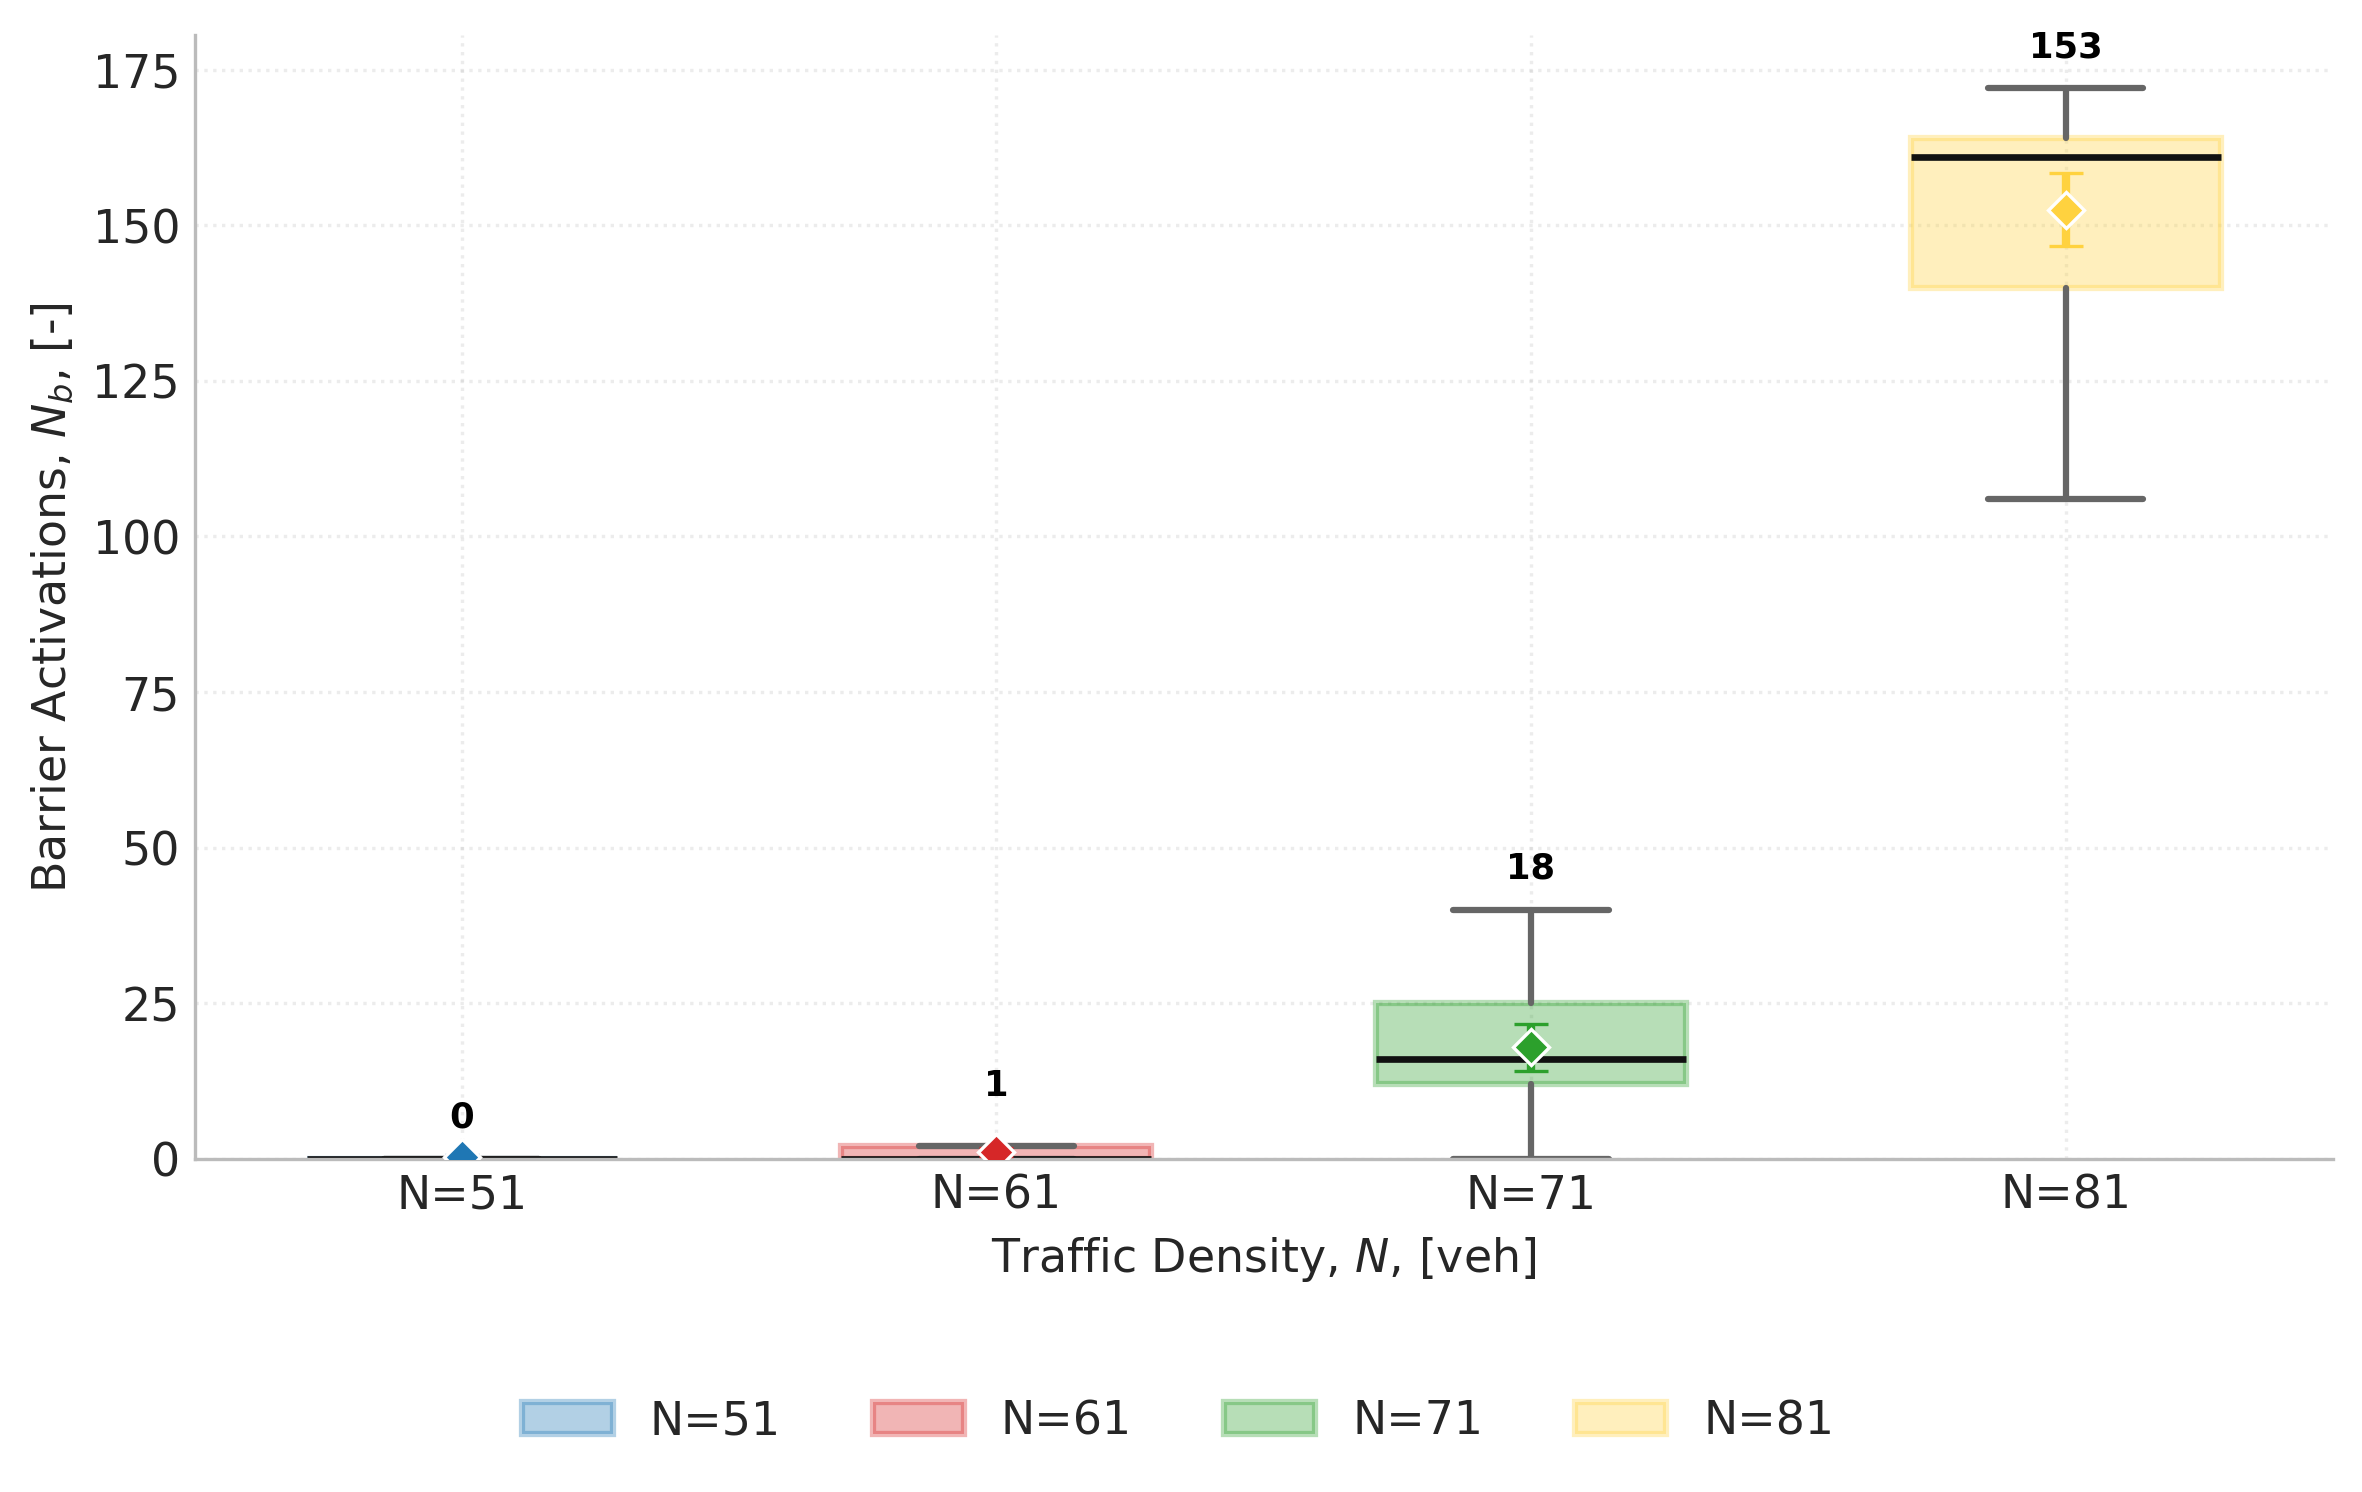
\includegraphics[height=4cm, keepaspectratio]{firings-per-demand.png}
        \caption{Boxplot indicating firings per traffic density \(N\), additional mean and 95\% CI are shown.}
        \label{fig:firings-per-demand}
    \end{subfigure}
    \hfill
    \begin{subfigure}[b]{0.48\textwidth}
        \centering
        % Matching height to ensure perfect alignment
        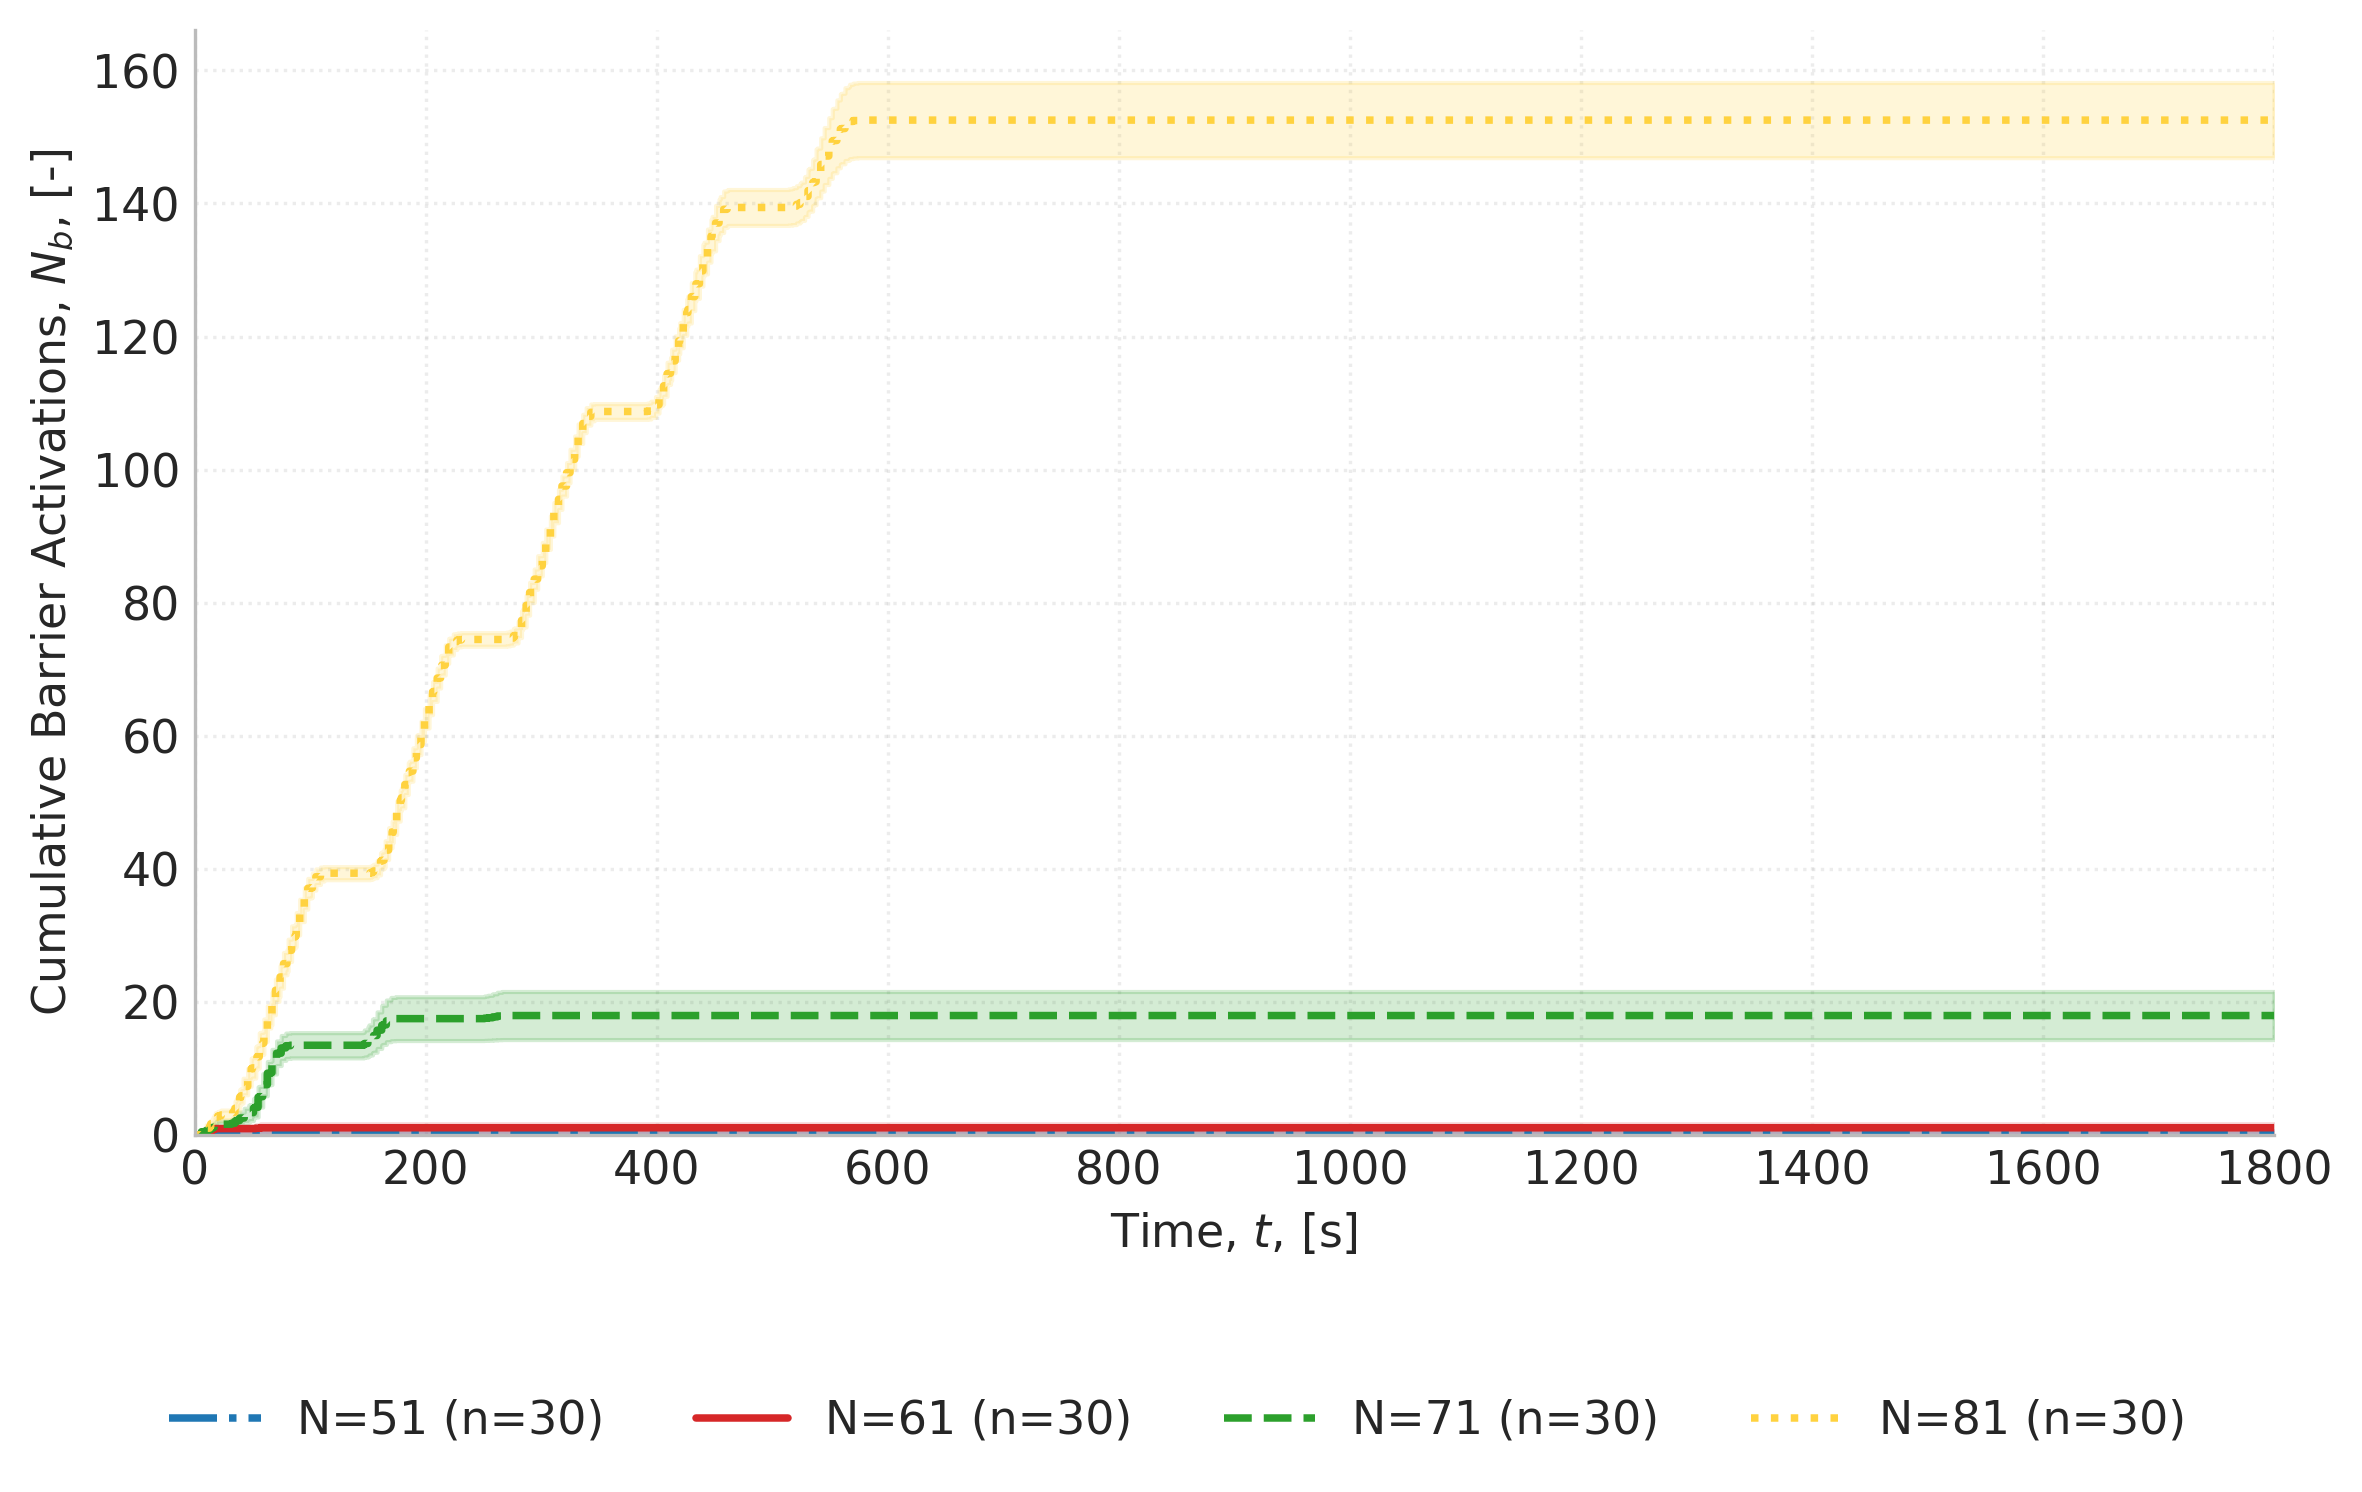
\includegraphics[height=4cm, keepaspectratio]{firings-over-time-all-demands.png}
        \caption{Cumulative firings over time for all traffic densities \(N\), displaying mean and 95\% CI.}
        \label{fig:firings-over-time}
    \end{subfigure}
    
    \caption{Analysis of barrier firings across different vehicle densities \(N = \{51,61,71,81\}\).}
    \label{fig:overall-firings-analysis}
\end{figure}
\subsection{KPI Comparison: Barrier vs. FAS}
This section describes the obtained differences in throughput, delay time, energy consumption, and safety violations from simulations.
 \subsubsection{Throughput}
 Figure~\ref{fig:throughput} displays the mean throughput for each simulation batch, and the error bars highlight the 95\% confidence interval, computed using the t-distribution. First, the figure shows no error bars, indicating that both controllers achieve identical throughput across the various number of runs. Second, the figure shows that the throughput achieved by the barrier controller exhibits a near-linear increase, from 0.36 veh/s at \(N=51\) to 0.57 at \(N=81\). On the other hand, the FAS controller shows a saturation point, around 0.32 veh/s beyond \(N=61\). In general, the barrier controller achieves higher throughput than the FAS controller across all \(N\), with throughput advantages of 34.75\%, 36.09\%, 61.00\% and 72.59\%, at \(N=51, 61, 71,\) and \(81\).   

\subsubsection{Delay Time}
Figure~\ref{fig:delayKPI} displays the mean cumulative delay time across various traffic densities. The figure demonstrates near-zero cumulative delay for the barrier controller across all traffic densities. Conversely, the FAS controller, demonstrates delay across all vehicle counts, ranging from 20000 s at \(N=51\) to 46500 s at \(N=81\). Overall, the barrier controller achieves a maximum decrease in delay time of 98.86\% relative to the FAS controller at \(N=81\).   



\subsubsection{Energy Consumption}
Figure~\ref{fig:energy} illustrates the mean energy consumption, standardized per km traveled. The barrier controller demonstrates near constant energy consumption of 0.077 kWh/km. It should be noted that at \(N=81\), energy consumption was slightly higher, 0.078 kWh/km.
In contrast, the FAS controller shows energy consumption ranging from 0.097 kWh/km at \(N=51\) all the way to 0.14 kWh/km at \(N=81\). Overall,  the barrier achieves energy reductions of 20.12\%, 22.85\%, 39.97\%, and 44.81\% at \(N=51, 61, 71,\) and \(81\).  


\subsubsection{Safety Violations}
Figure~\ref{fig:safetycounting} displays the mean safety violations per traffic density. Both controllers show zero safety violations at \(N=\{51,61\}\). Whereas, the FAS controller continues with near-zero violations at \(N=\{71,81\}\), the barrier controller records  1.9±0.82 violations per run at \(N=71\), and 21.13±1.69 violations per run at \(N=81\). Despite these counted safety violations, figure~\ref{fig:safety-violations-time} shows that the violations only occur during the non steady-state phase. Once steady-state is reached, no further violations occur. 

\begin{figure}[H]
    \centering
    % Row 1
    \begin{subfigure}[b]{0.48\textwidth}
        \centering
        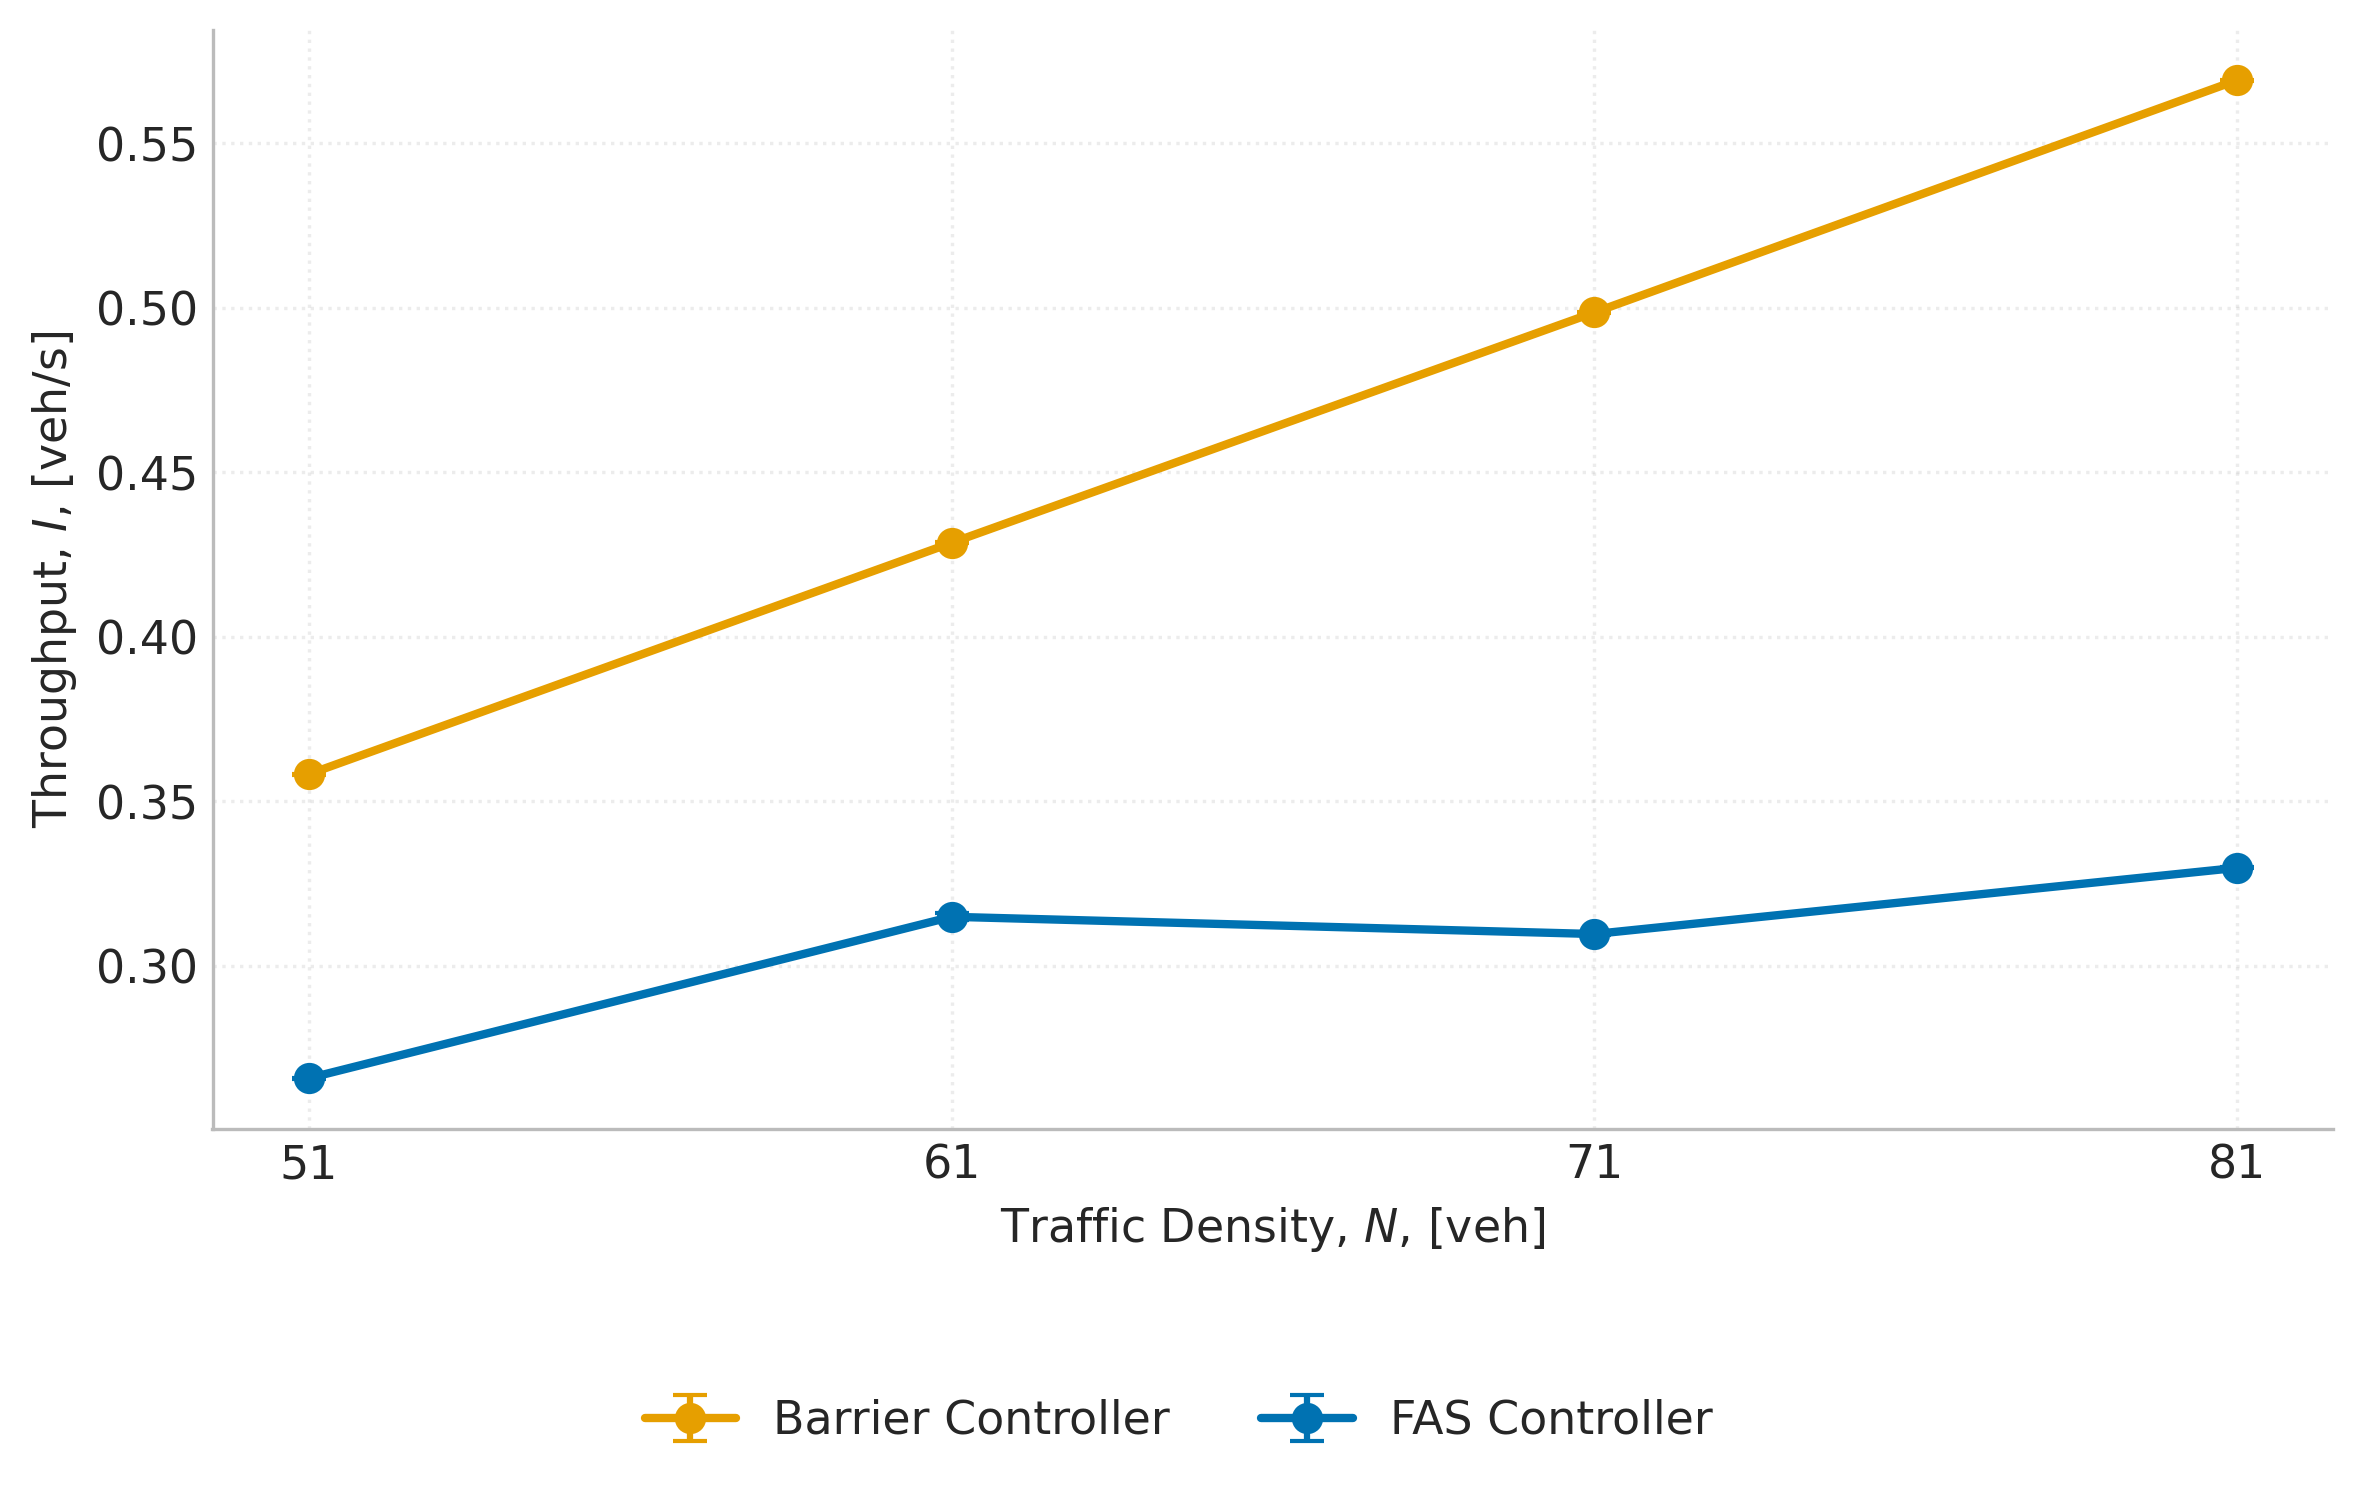
\includegraphics[width=\textwidth]{throughput-veh-s.png}
        \caption{Throughput}
        \label{fig:throughput}
    \end{subfigure}
    \hfill
    \begin{subfigure}[b]{0.48\textwidth}
        \centering
        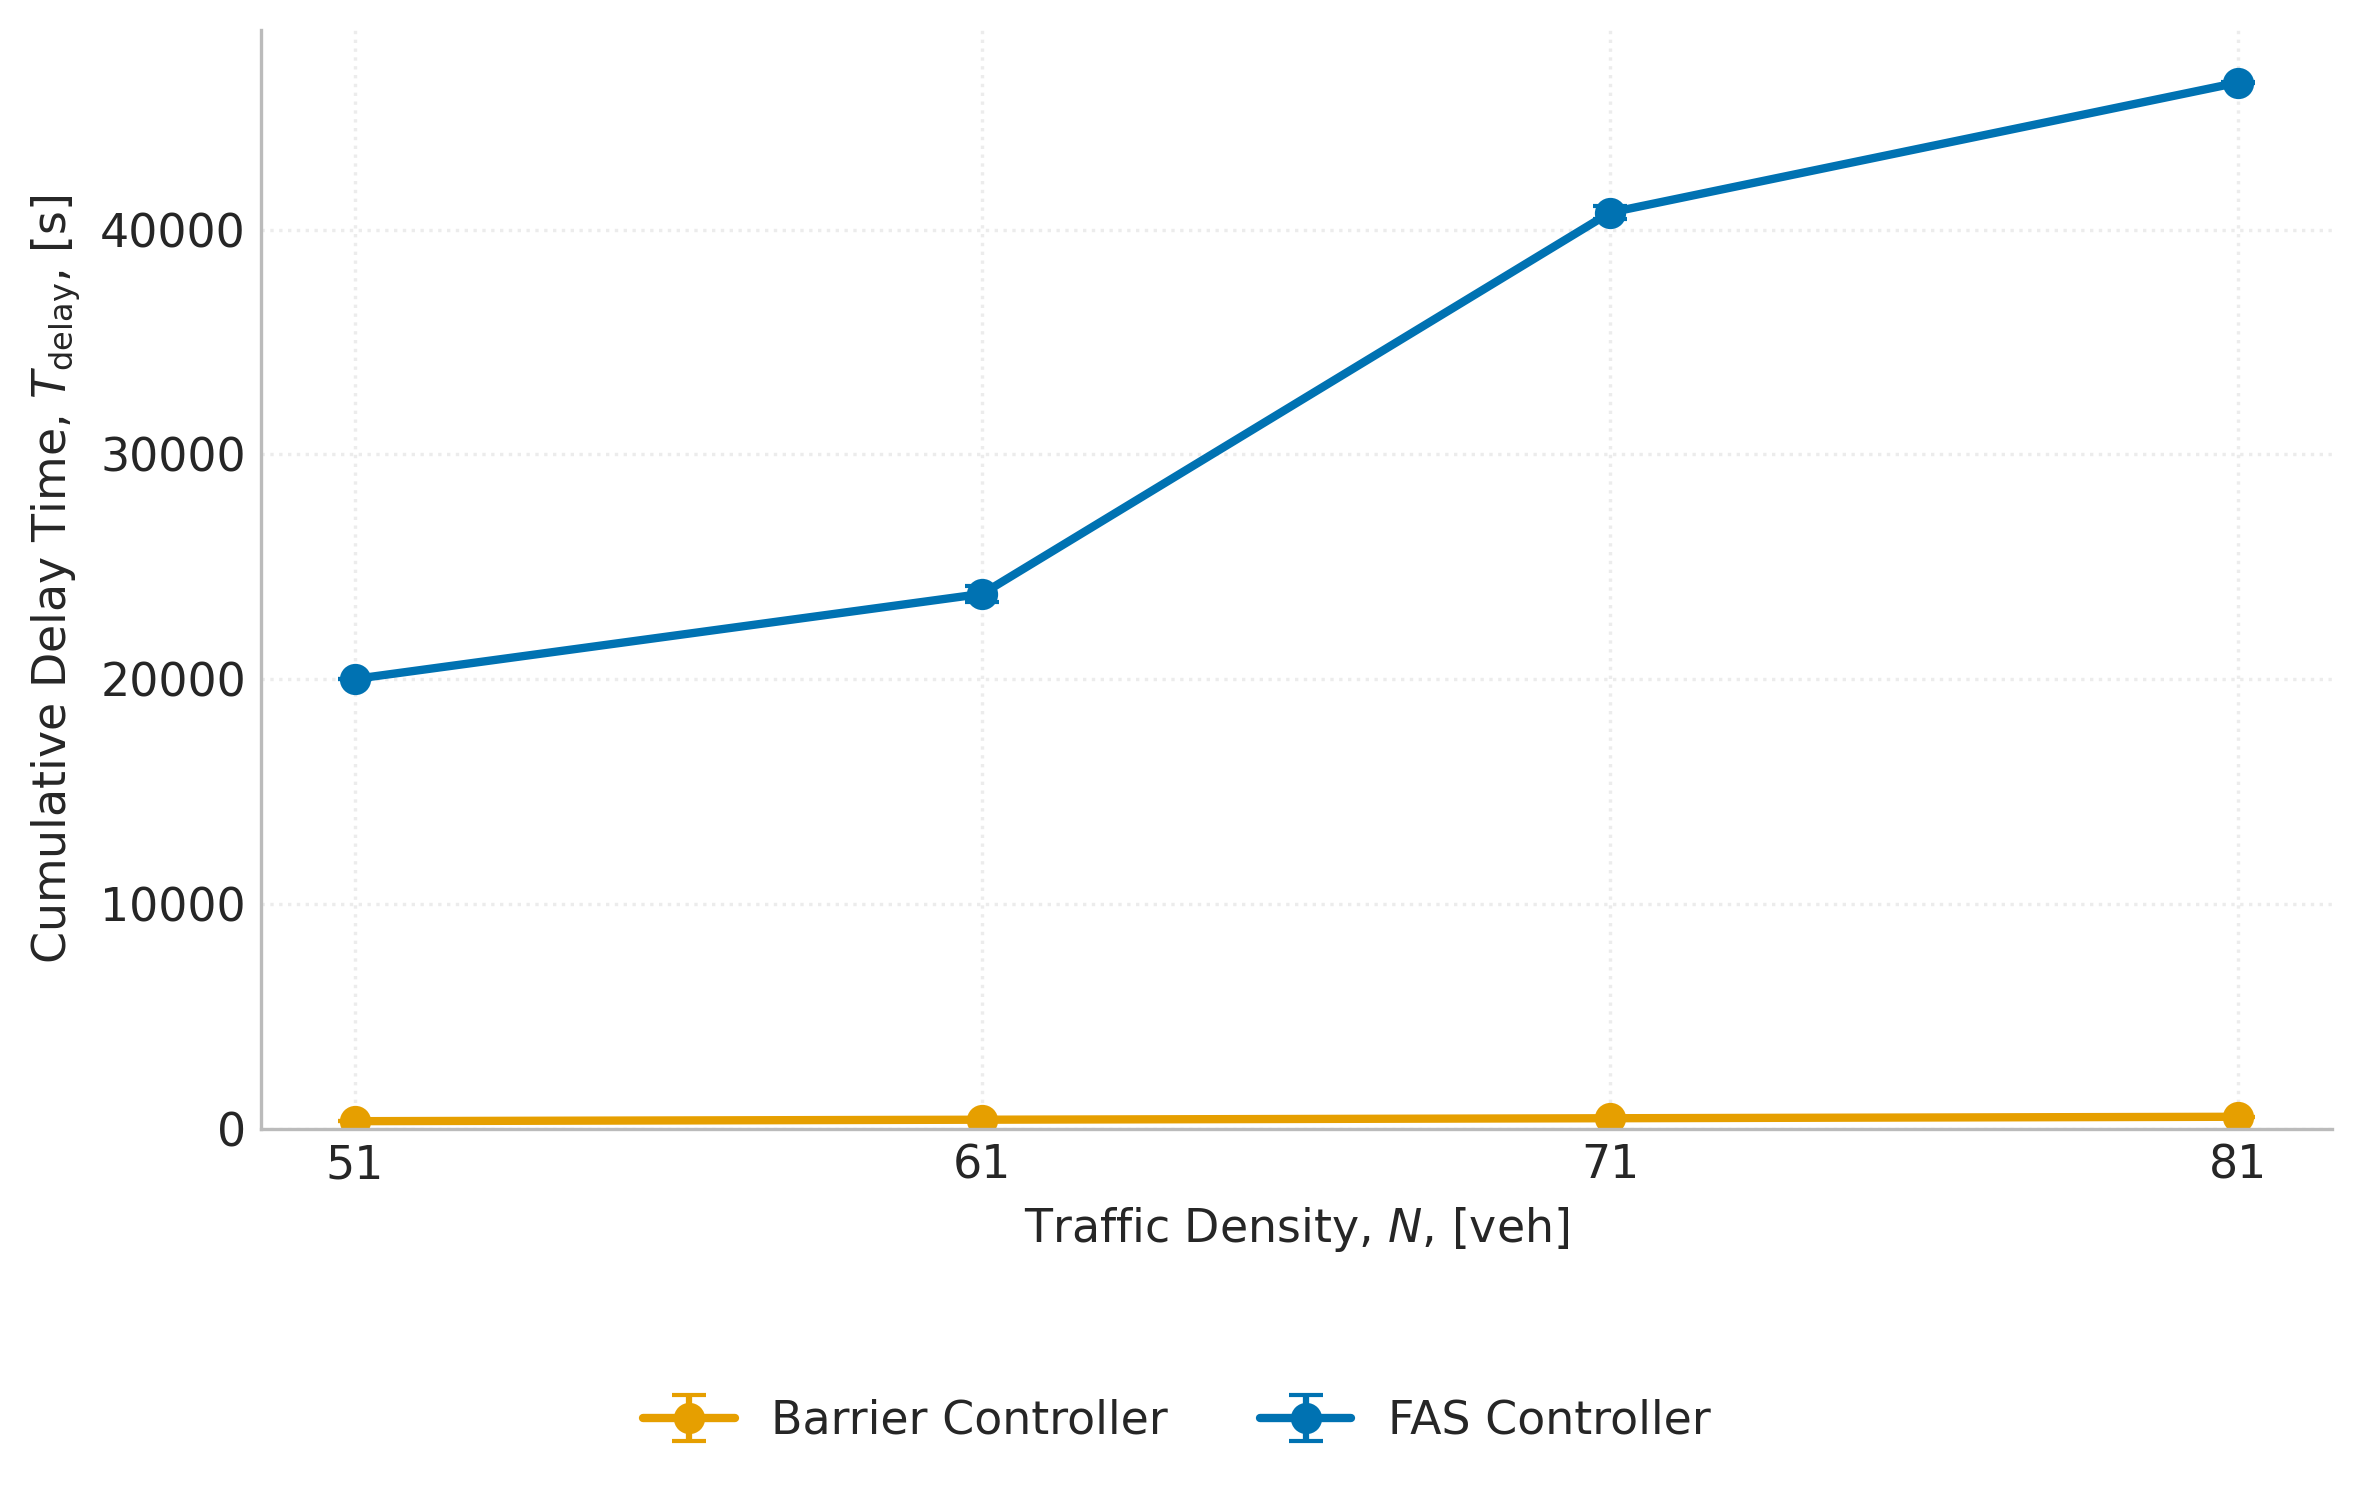
\includegraphics[width=\textwidth]{delay-s.png}
        \caption{Delay Time}
        \label{fig:delayKPI}
    \end{subfigure}
    
    \vspace{10pt} % Adds vertical spacing between the rows
    
    % Row 2
    \begin{subfigure}[b]{0.48\textwidth}
        \centering
        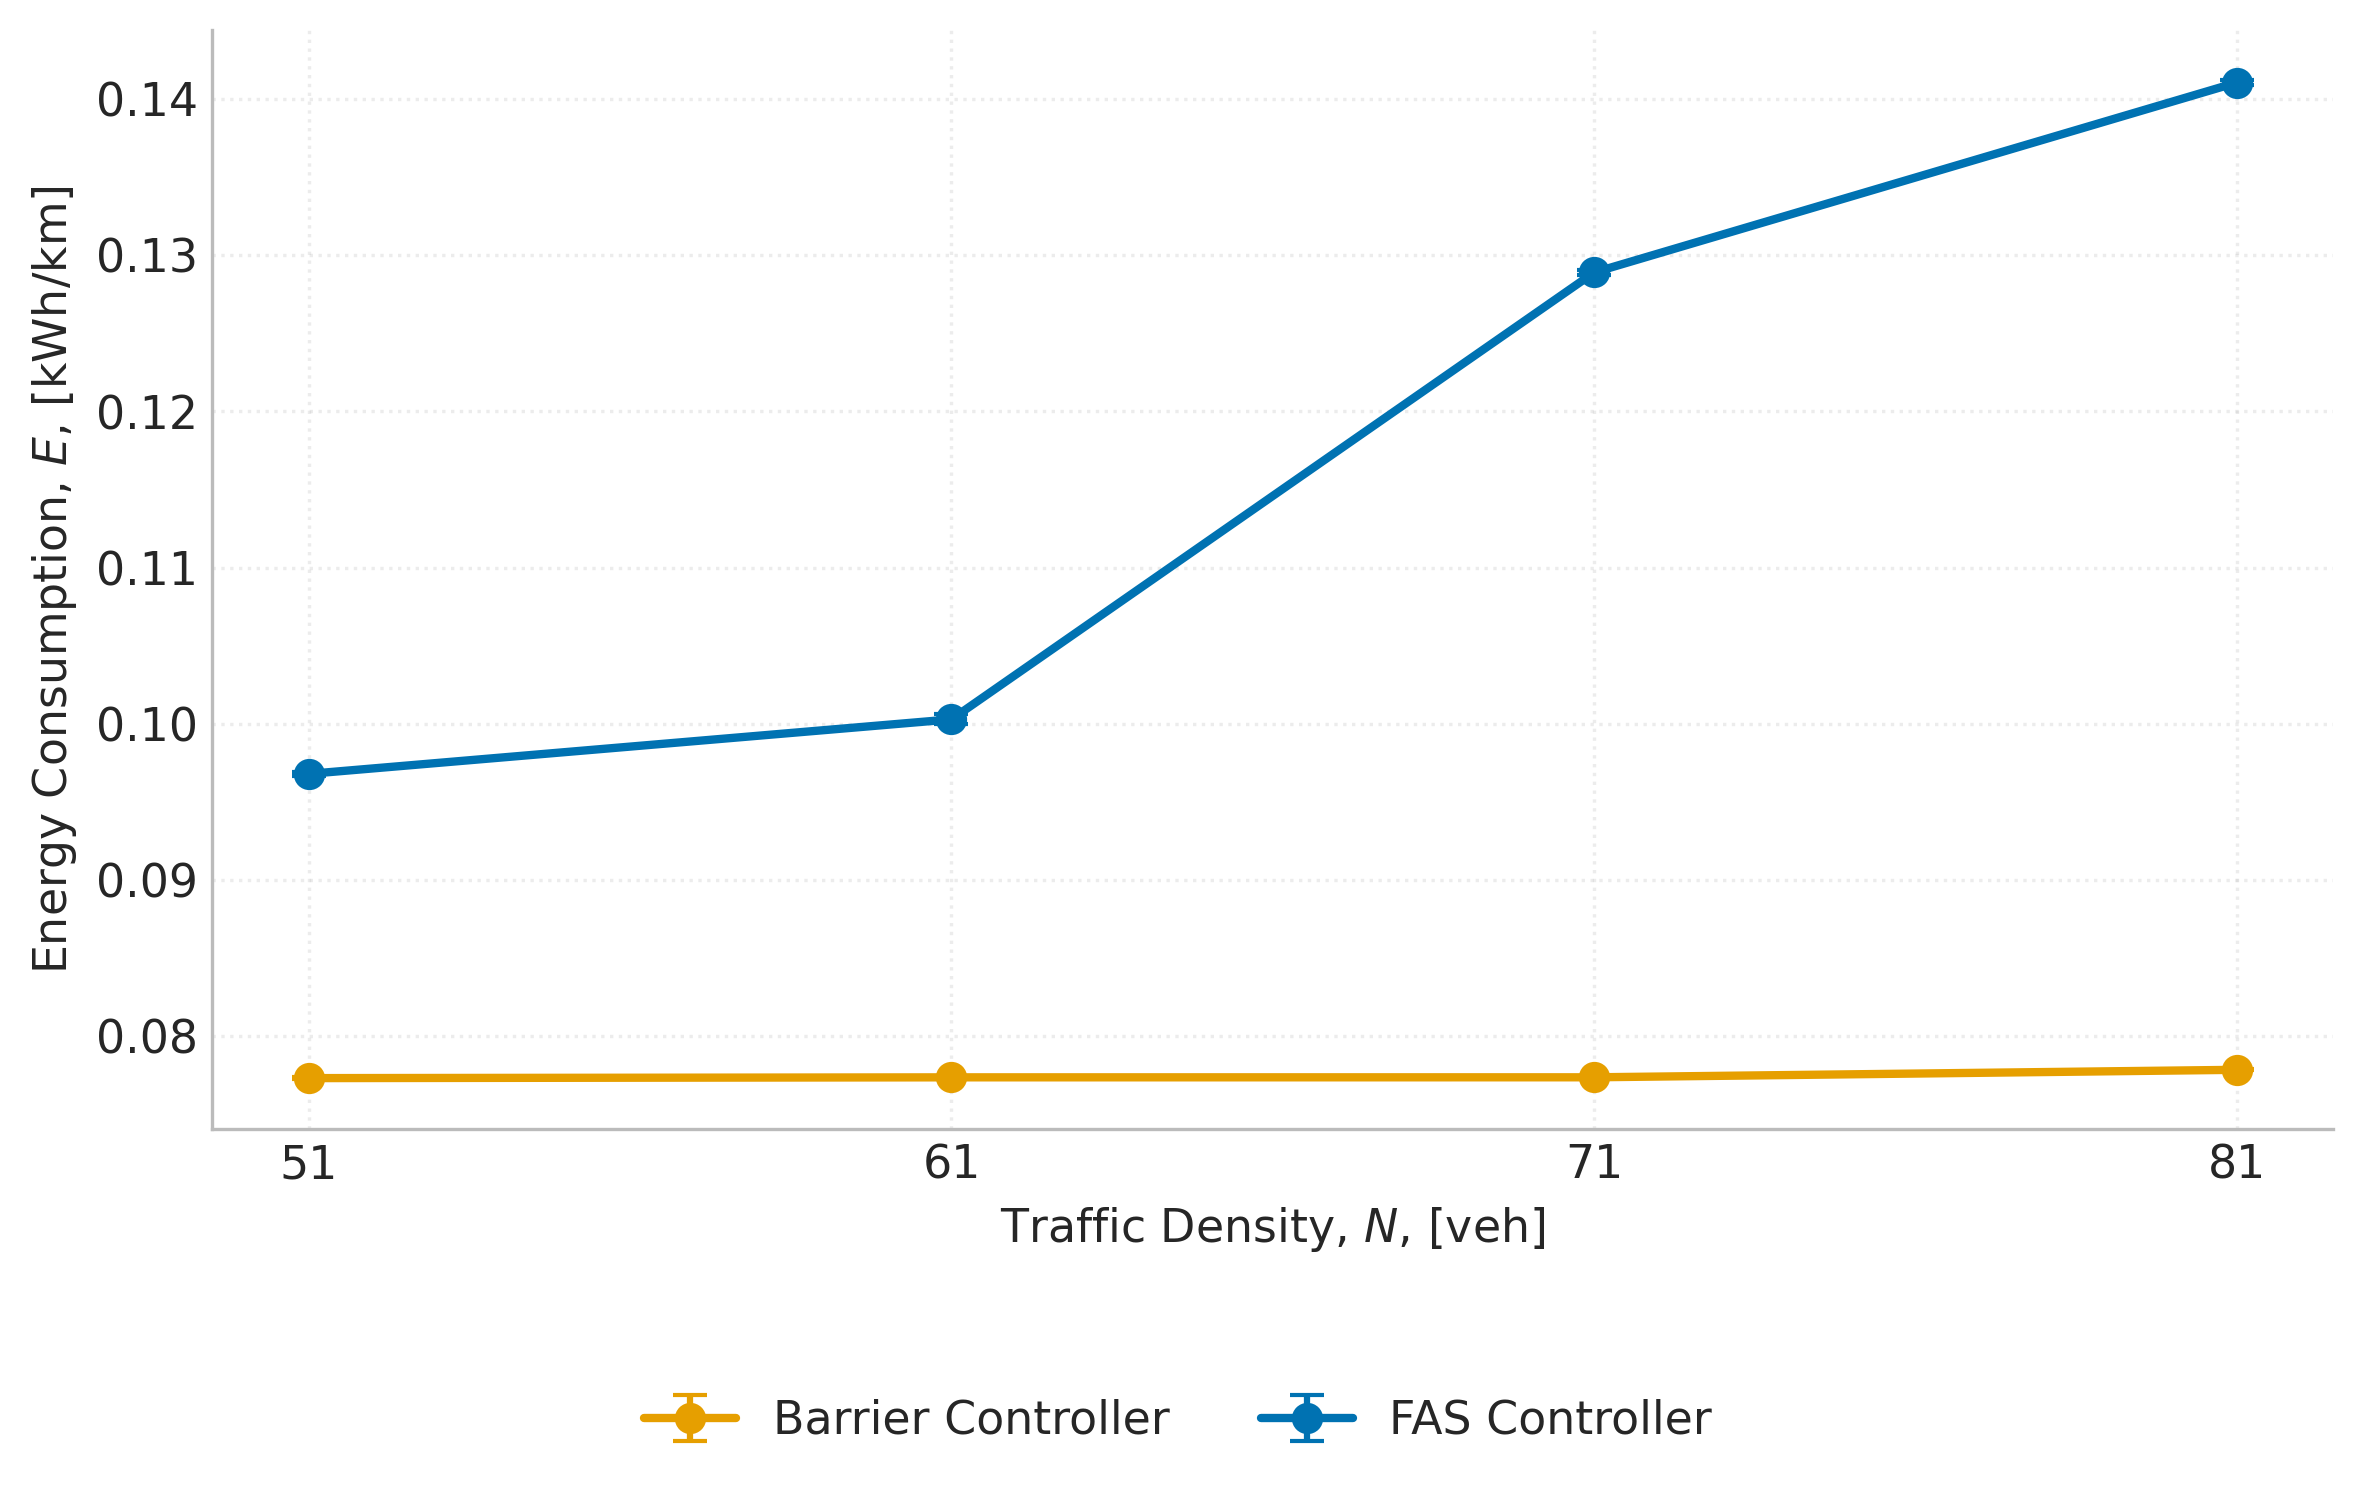
\includegraphics[width=\textwidth]{energy-kwh-per-km.png}
        \caption{Energy Consumption}
        \label{fig:energy}
    \end{subfigure}
    \hfill
    \begin{subfigure}[b]{0.48\textwidth}
        \centering
        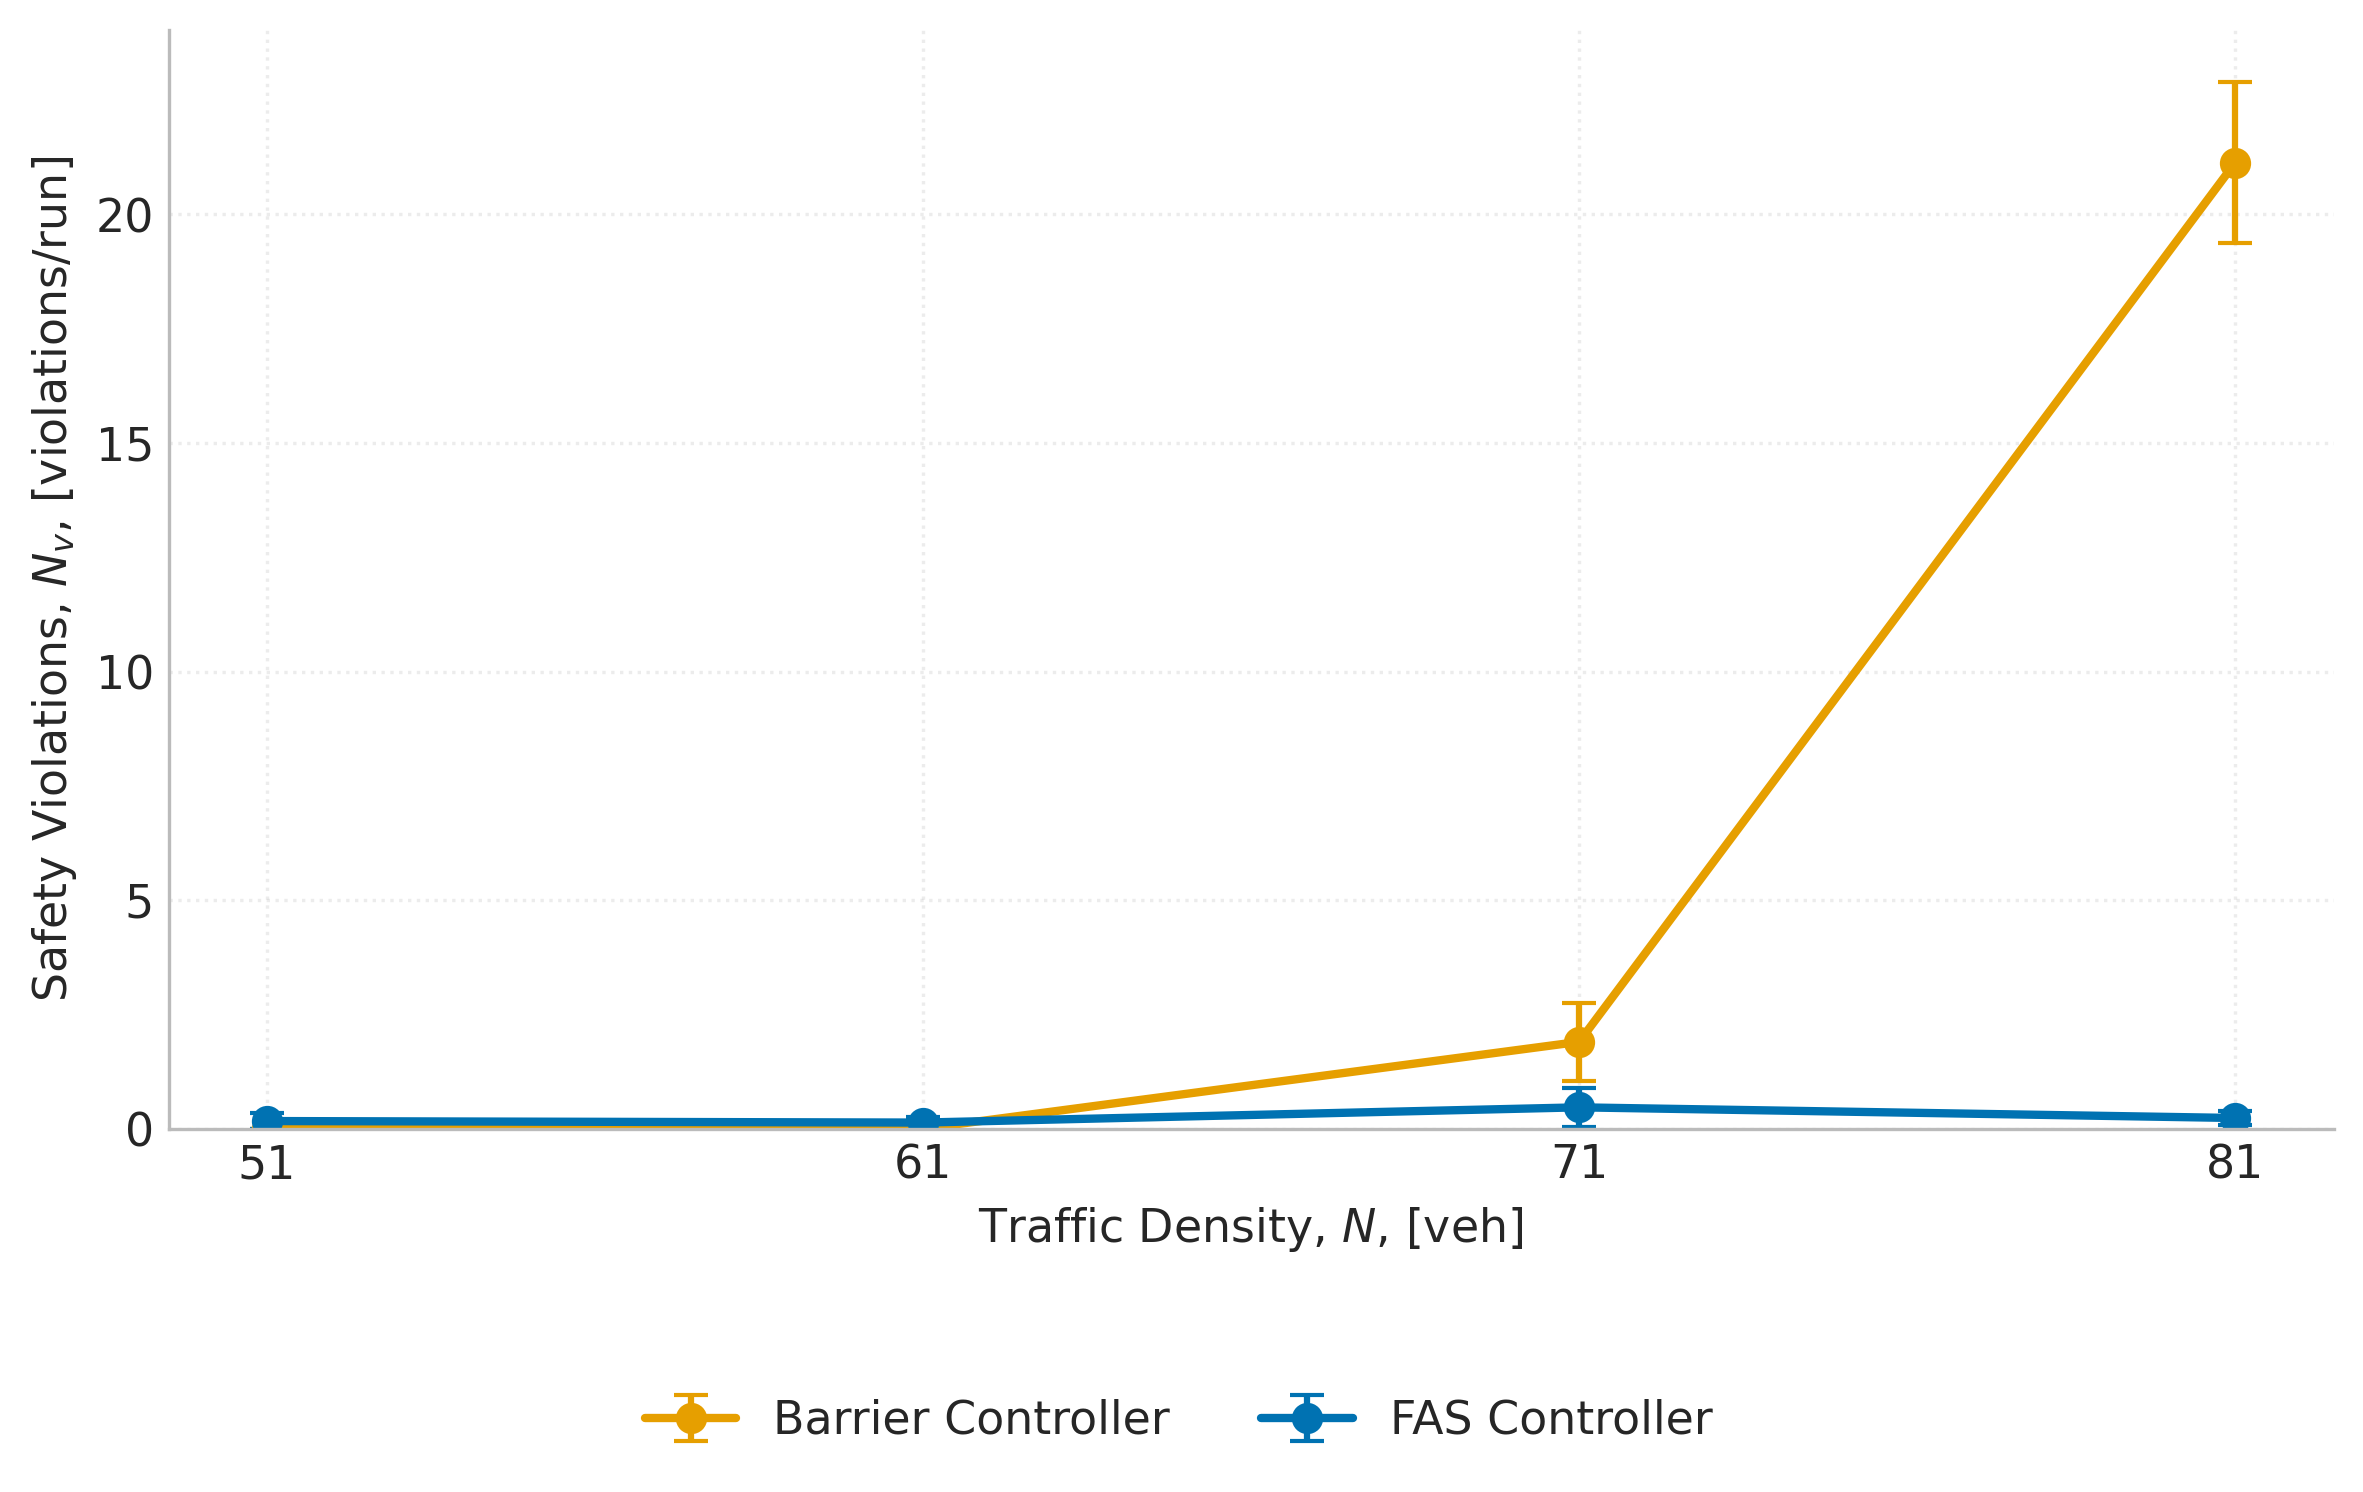
\includegraphics[width=\textwidth]{safety-violations-count.png}
        \caption{Safety Violations}
        \label{fig:safetycounting}
    \end{subfigure}
    
    \caption{Comparison of key performance indicators across traffic densities $N=\{51,61,71,81\}$, showing mean and 95\% CI.}
    \label{fig:kpi-four-metrics}
\end{figure}
\begin{figure}[H]
    \centering
    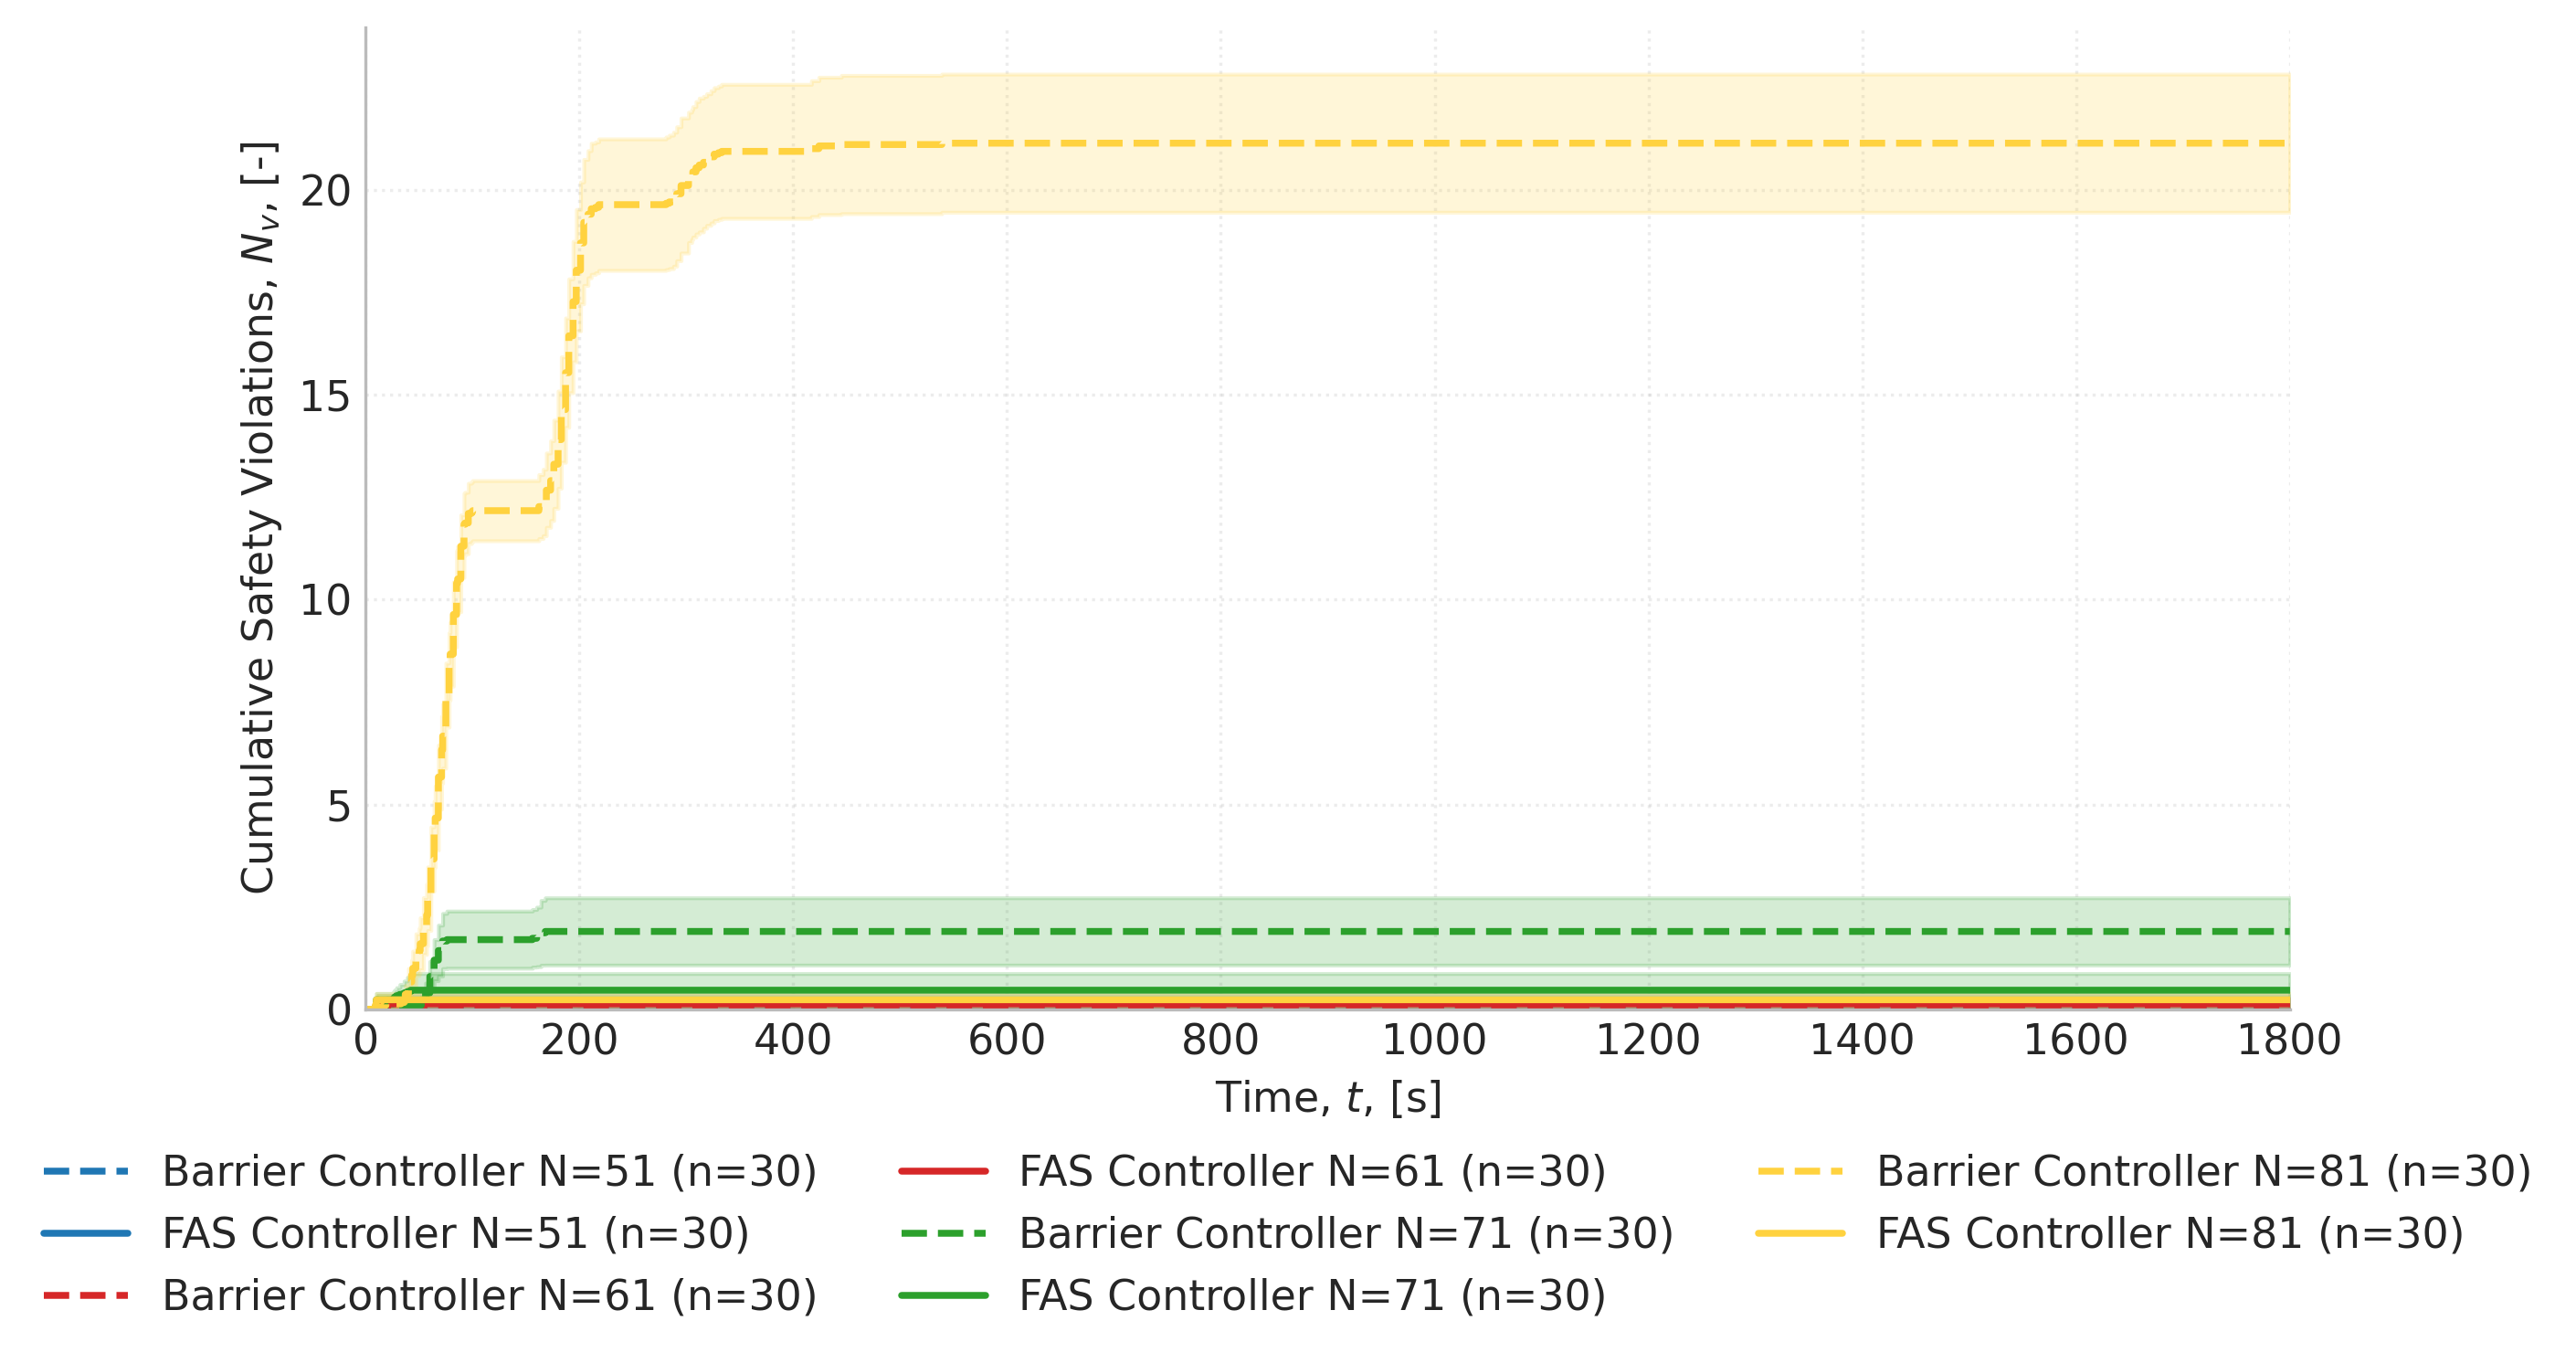
\includegraphics[width=\linewidth]{safety-violations-over-time.png}
    \caption{Cumulative safety violations over time across traffic densities \(N\ =\{51,61,71,81\}\), showing mean and 95\% CI.}
    \label{fig:safety-violations-time}
\end{figure}